\documentclass[aspectratio=169]{beamer}

% Packages
\usepackage{amsmath, amsfonts, amssymb}
\usepackage{graphicx}
\usepackage{hyperref}
\usepackage{booktabs}
\usepackage{bm}
\usepackage{algorithm}
\usepackage[noend]{algpseudocode}
\usepackage{listings}
\usepackage{xcolor}
\usepackage{tikz}
\usepackage{color}

\usetheme{Madrid} % You can choose any theme you like
\usecolortheme{default}

% 定义自定义颜色
\definecolor{darkprimary}{HTML}{00796B}
\definecolor{lightprimary}{HTML}{B2DFDB}
\definecolor{primary}{HTML}{009688}
\definecolor{texticons}{HTML}{FFFFFF}
\definecolor{accent}{HTML}{FFC107}
\definecolor{primarytext}{HTML}{212121}
\definecolor{secondarytext}{HTML}{757575}
\definecolor{divider}{HTML}{BDBDBD}

% 设置颜色
\setbeamercolor{structure}{fg=primary}
\setbeamercolor{normal text}{fg=primarytext, bg=lightprimary}
\setbeamercolor{frametitle}{fg=texticons, bg=darkprimary}
\setbeamercolor{item}{fg=accent}
\setbeamercolor{block title}{bg=darkprimary, fg=texticons}
\setbeamercolor{block body}{bg=lightprimary, fg=primarytext}

% Adjust global spacing
\setlength{\parskip}{0.1em}
\setlength{\itemsep}{0.1em}
\setlength{\columnsep}{0.3em}
\setlength{\abovecaptionskip}{0.1em}
\setlength{\belowcaptionskip}{0.1em}
\setbeamersize{text margin left=0.3em, text margin right=0.3em}

\setbeamertemplate{navigation symbols}{} % Remove navigation symbols

% Title Page Details
\title[ML Sentiment Analysis for Finance]{Machine Learning Based Sentiment Analysis of Financial Texts}
\author[C.J., B.L. and S.S.]{Chuan Jia, Bo Li and Sheng Su*}
\institute[M.U.S.T.]{Macau University of Science and Technology}
\date{December 14, 2024}

% Logo (Placeholder)
\titlegraphic{
\includegraphics[height=1.5cm]{logo.png}} % Replace 'logo.png' with your school logo file

\begin{document}

% Cover Slide
\begin{frame}
    \titlepage
    \vspace{0.4cm} % Adjust spacing as needed
    \footnotesize{\textit{*Note: The order of authors' names follows the alphabetical order of their last names.}}
\end{frame}

%-----------------------------------------------
% Problem Statement (1 slides)
%-----------------------------------------------
\begin{frame}{Problem Statement}
\textbf{Background:}
\begin{itemize}
  \item \underline{Massive volumes of financial text} (news, reports, social media) influence investment decisions.
  \item Traditional analysis often \underline{overlooks subtle emotional cues} embedded in textual data.
  \item \underline{Objective:} Integrate sentiment analysis into financial decision-making to enhance rationality and predictive accuracy.
\end{itemize}

\textbf{Objectives:}
\begin{itemize}
  \item \underline{Challenge:} Limited high-quality, annotated Chinese financial sentiment corpora.
  \item \underline{Need:} A robust methodology to generate and leverage domain-specific labeled datasets.
  \item \underline{Goal:} Improve Chinese financial sentiment classification via data augmentation and Transformer-based models.
\end{itemize}
\end{frame}

%-----------------------------------------------
% Methods (2 slides)
%-----------------------------------------------
\begin{frame}{Dataset Describtion}
  \textbf{Dataset Overview:}
  \begin{itemize}
    \item \underline{Extended Chinese financial news articles} from \textit{Various Sources}.
    \item \underline{Sentiment Labels:} Positive, Neutral, Negative.
    \item \underline{Size:} 54749 labeled articles.
  \end{itemize}
  
  \textbf{Data Preprocessing:}
  \begin{itemize}
    \item \underline{Extension:} Translated high-quality labeled English financial sentiment corpora into Chinese.
    \item \underline{Prelabel:} Used a Chinese financial sentiment lexicon for non-labeled data.
    \item \underline{Tokenization:} Jieba Chinese tokenizer.
  \end{itemize}
\end{frame}

\begin{frame}{Dataset Visualization}
  \begin{columns}[t]
      \column{0.5\textwidth}
      \textbf{Sentiment Distribution:}
      \begin{figure}
          \centering
          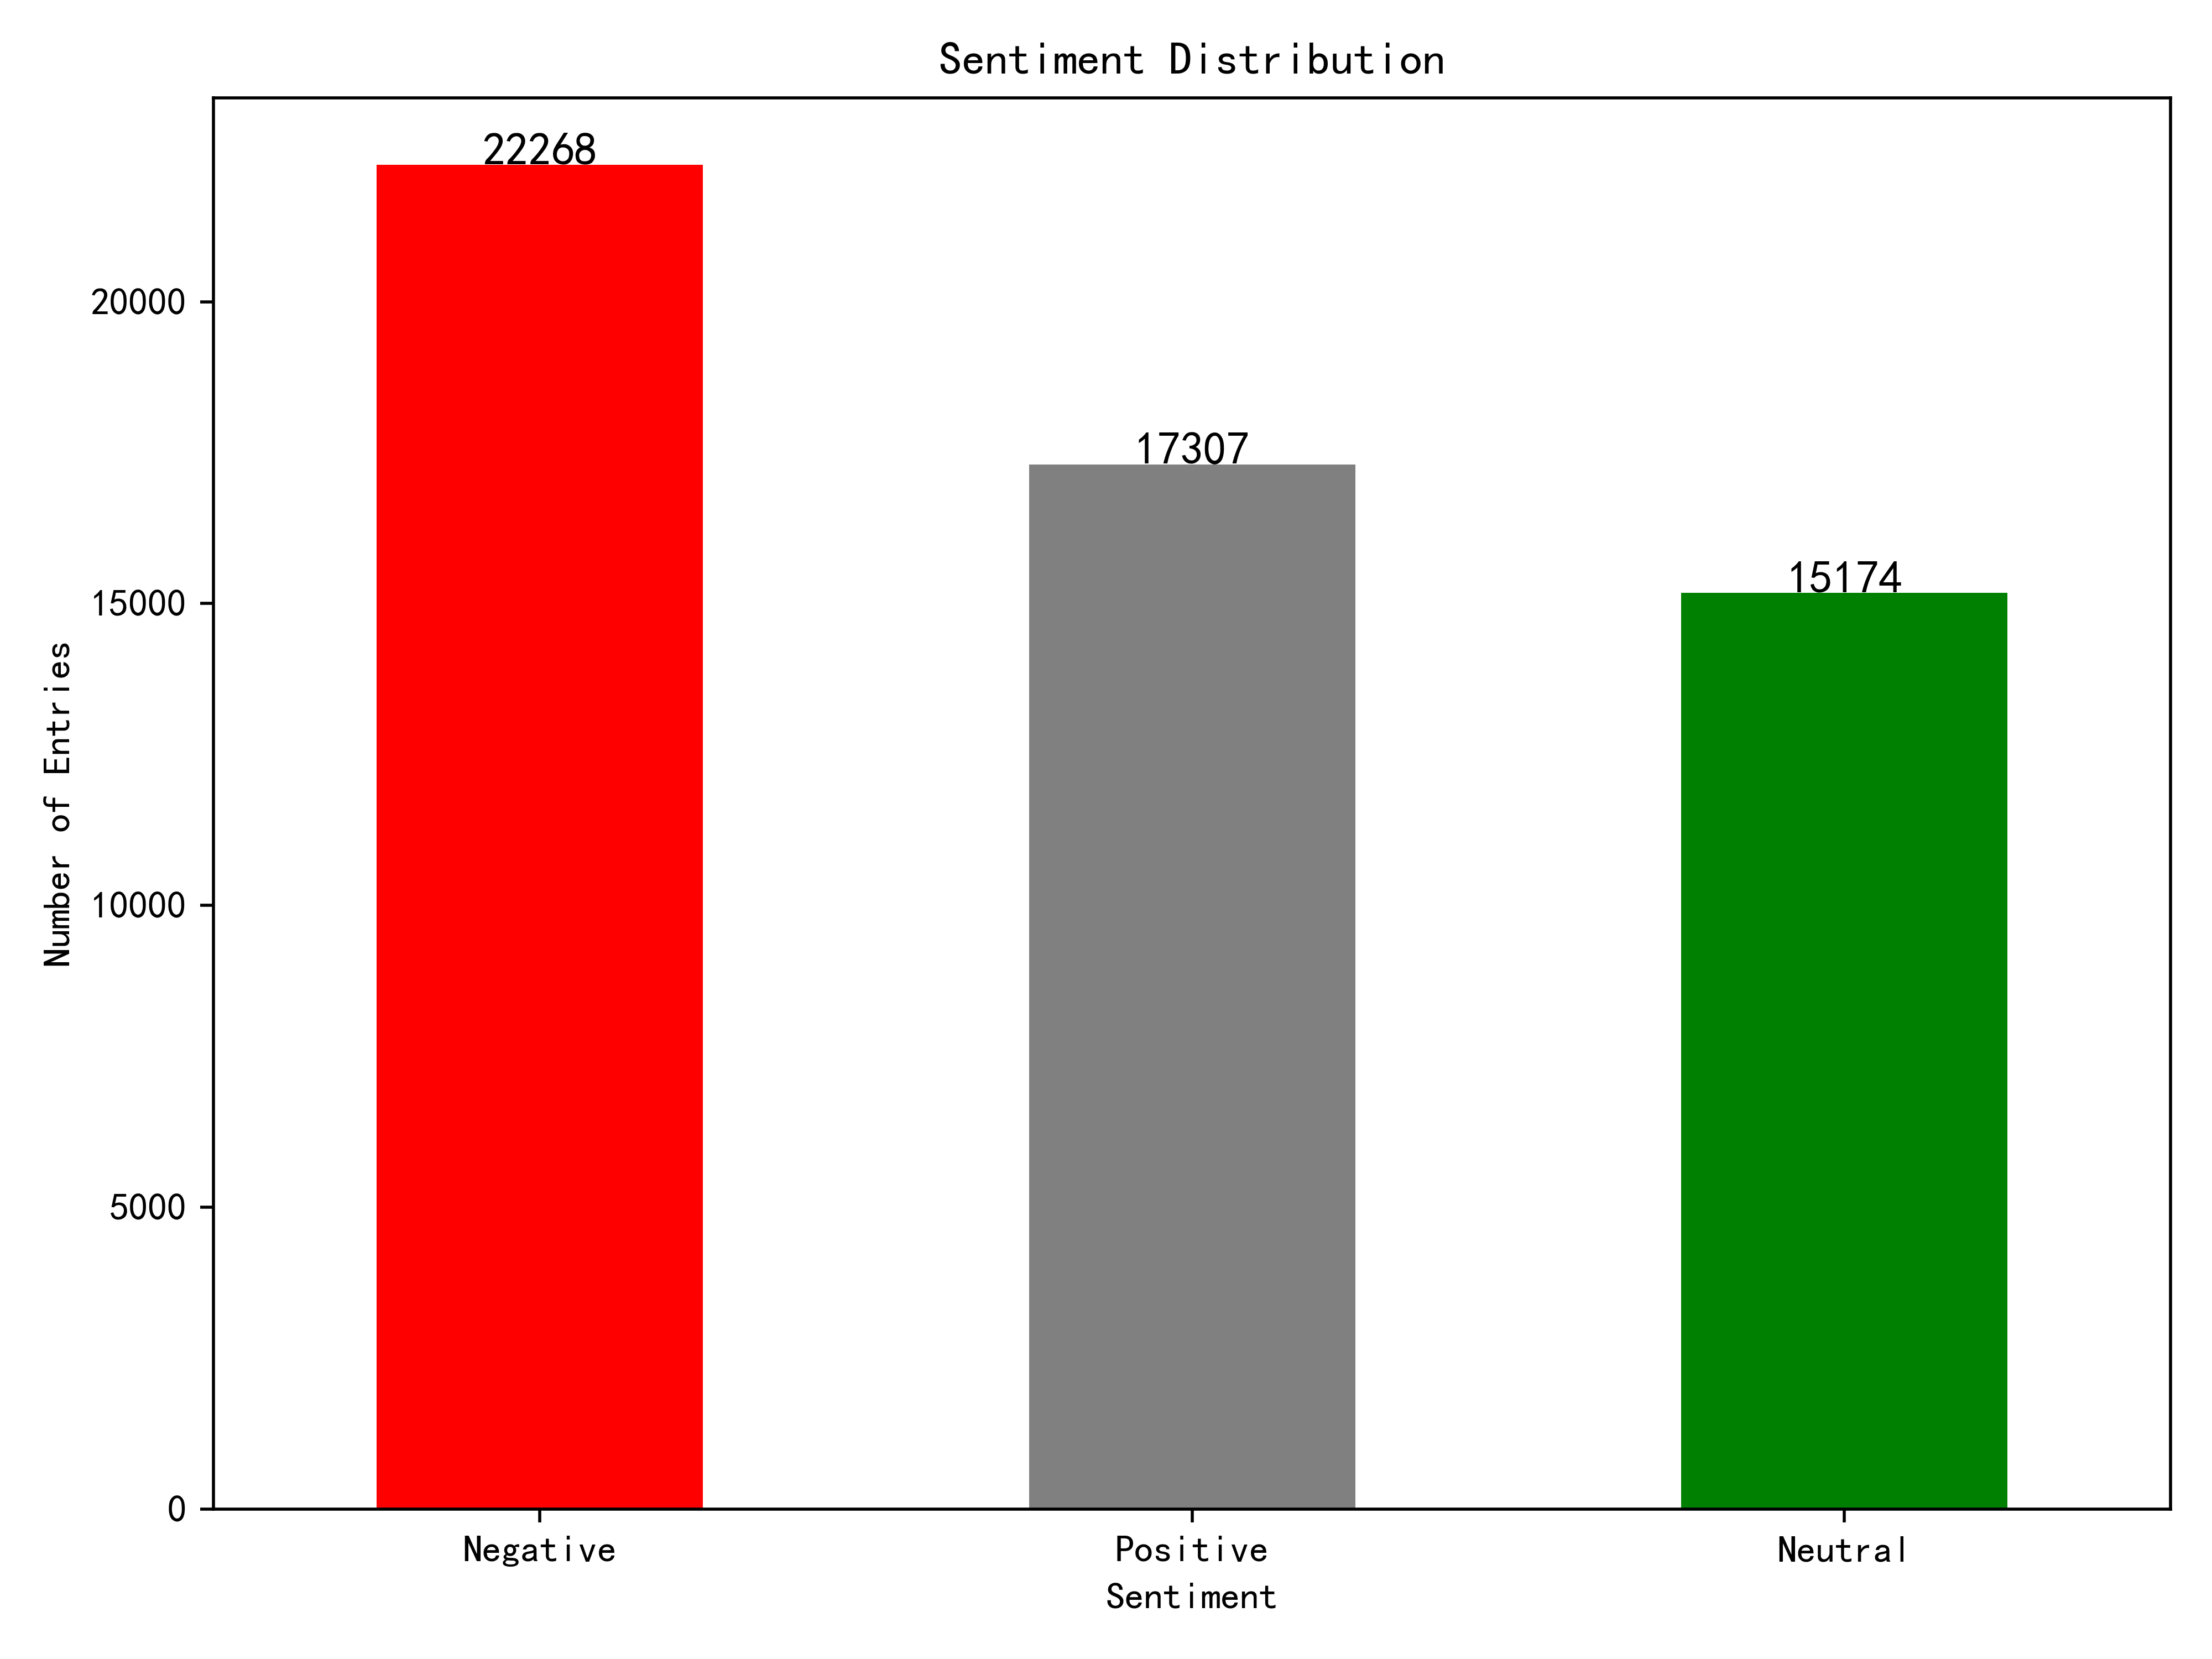
\includegraphics[width=\linewidth]{sentiment_distribution.png}
          \caption{Distribution of Sentiments}
      \end{figure}
  \end{columns}
\end{frame}

\begin{frame}{Dataset Visualization (Continue)}
  \textbf{Word Clouds:}
  \begin{figure}
    \centering
    % Top: Neutral sentiment
    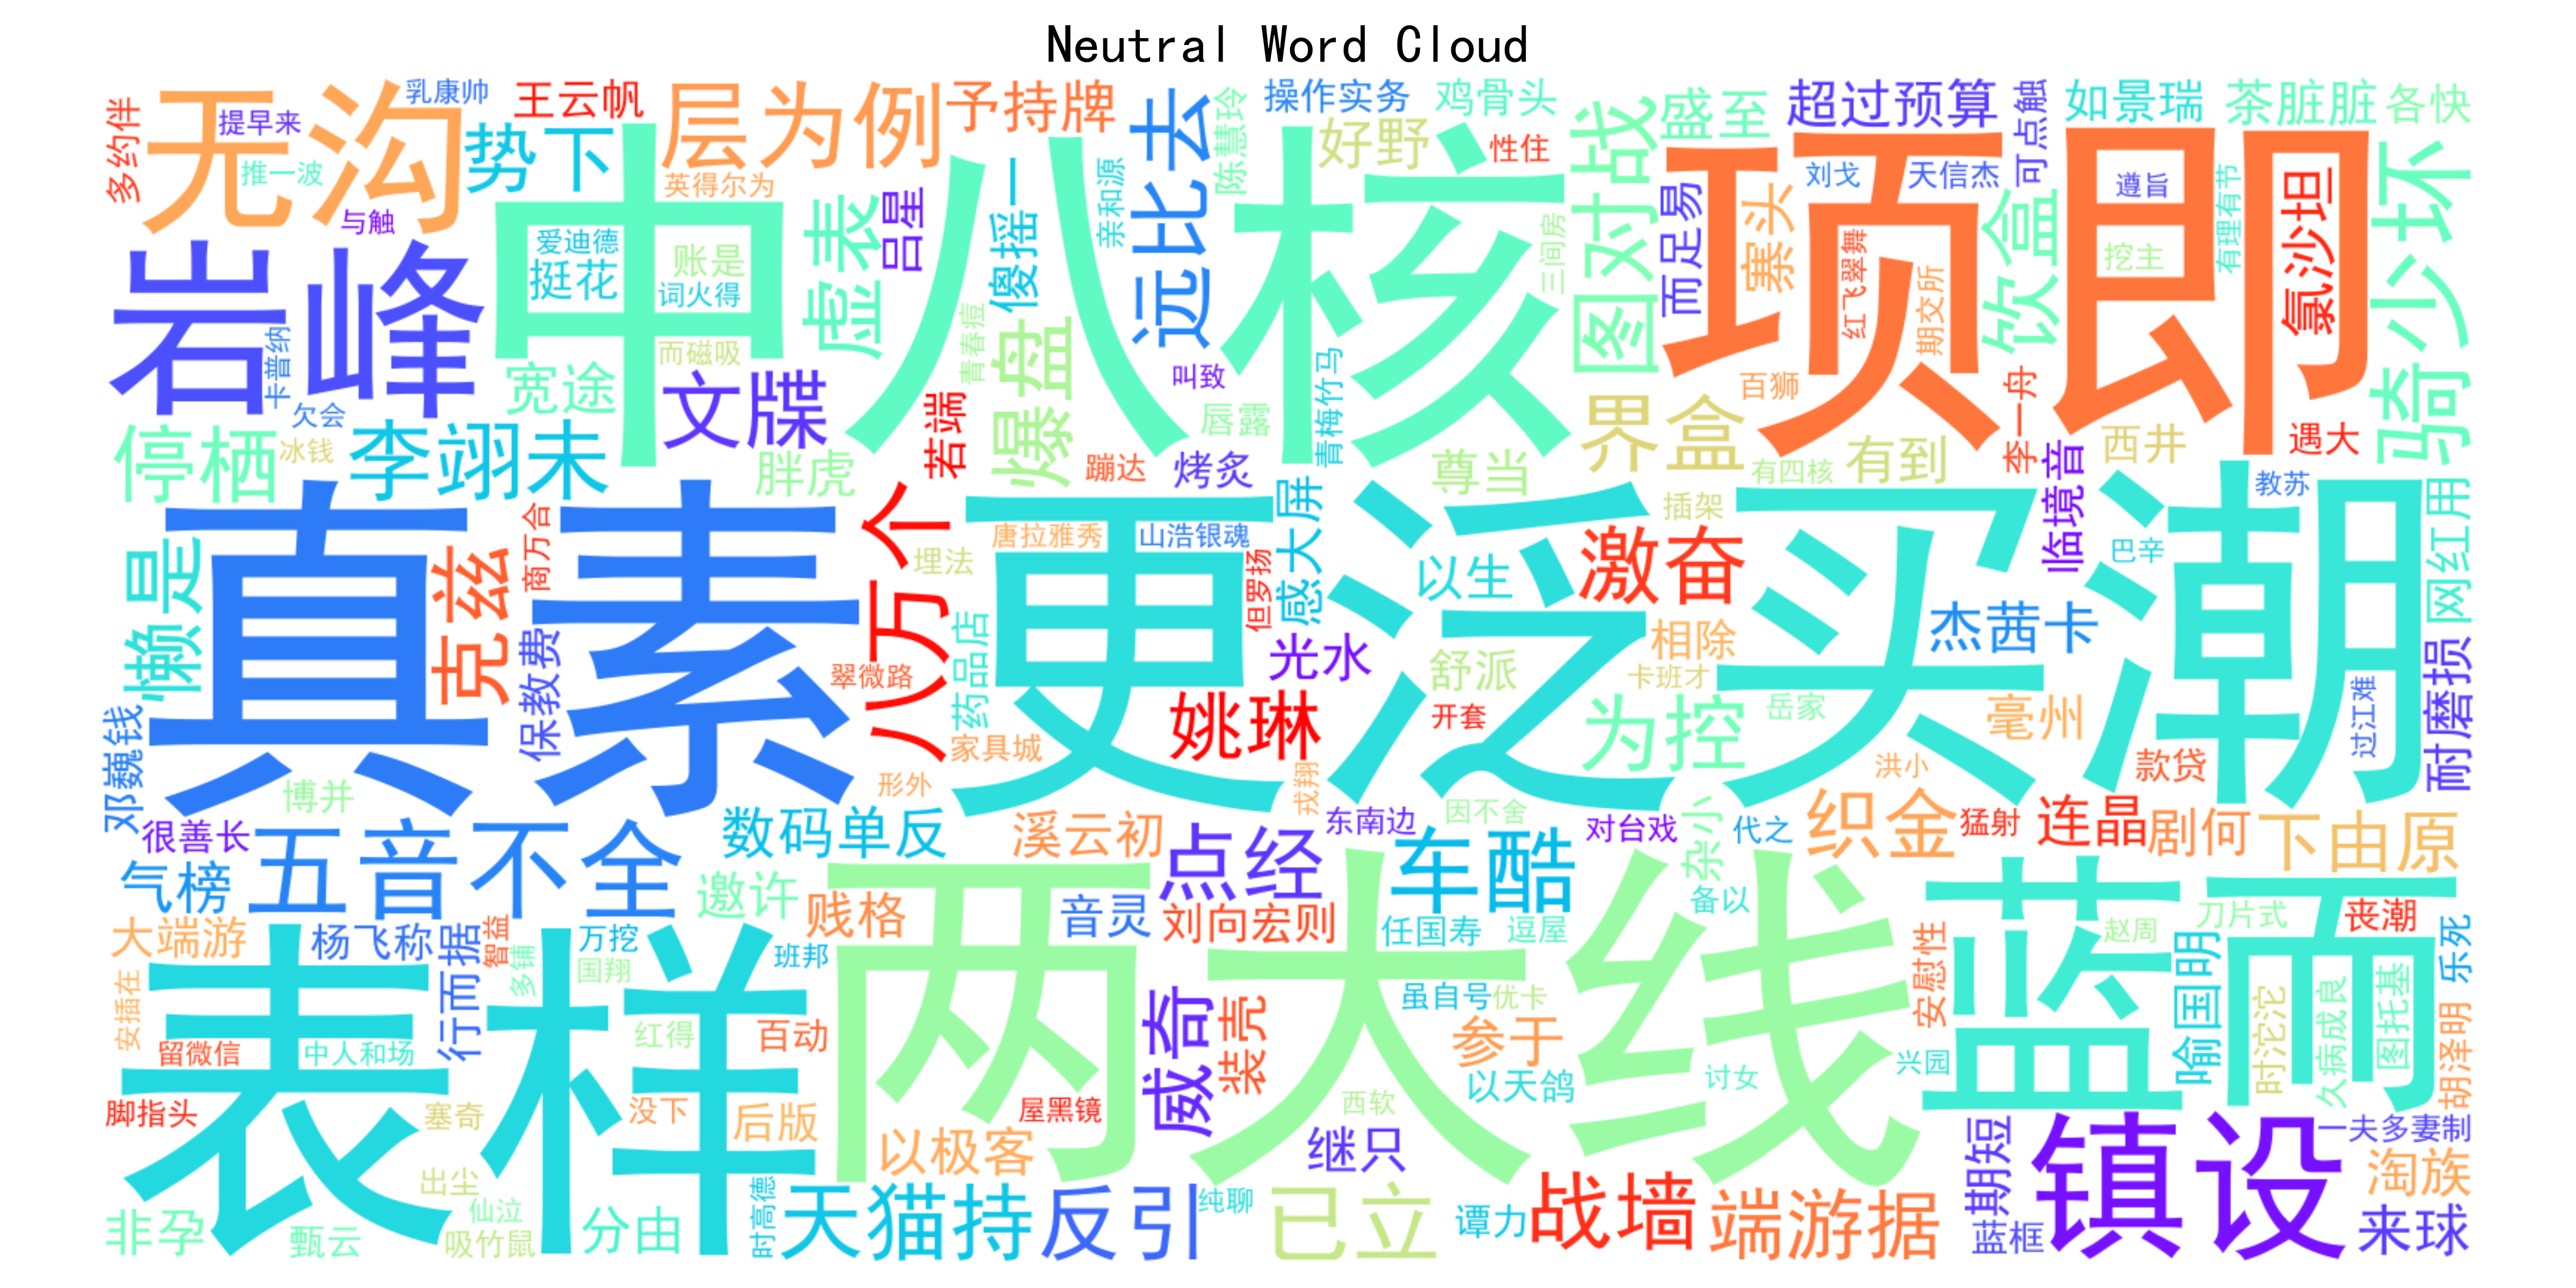
\includegraphics[width=0.33\linewidth]{wordcloud_neutral.png}
    \caption{\small Neutral Sentiment}
    \vspace{1em}

    % Bottom: Positive and Negative sentiments side-by-side
    \begin{columns}[c]
      \column{0.5\textwidth}
      \centering
      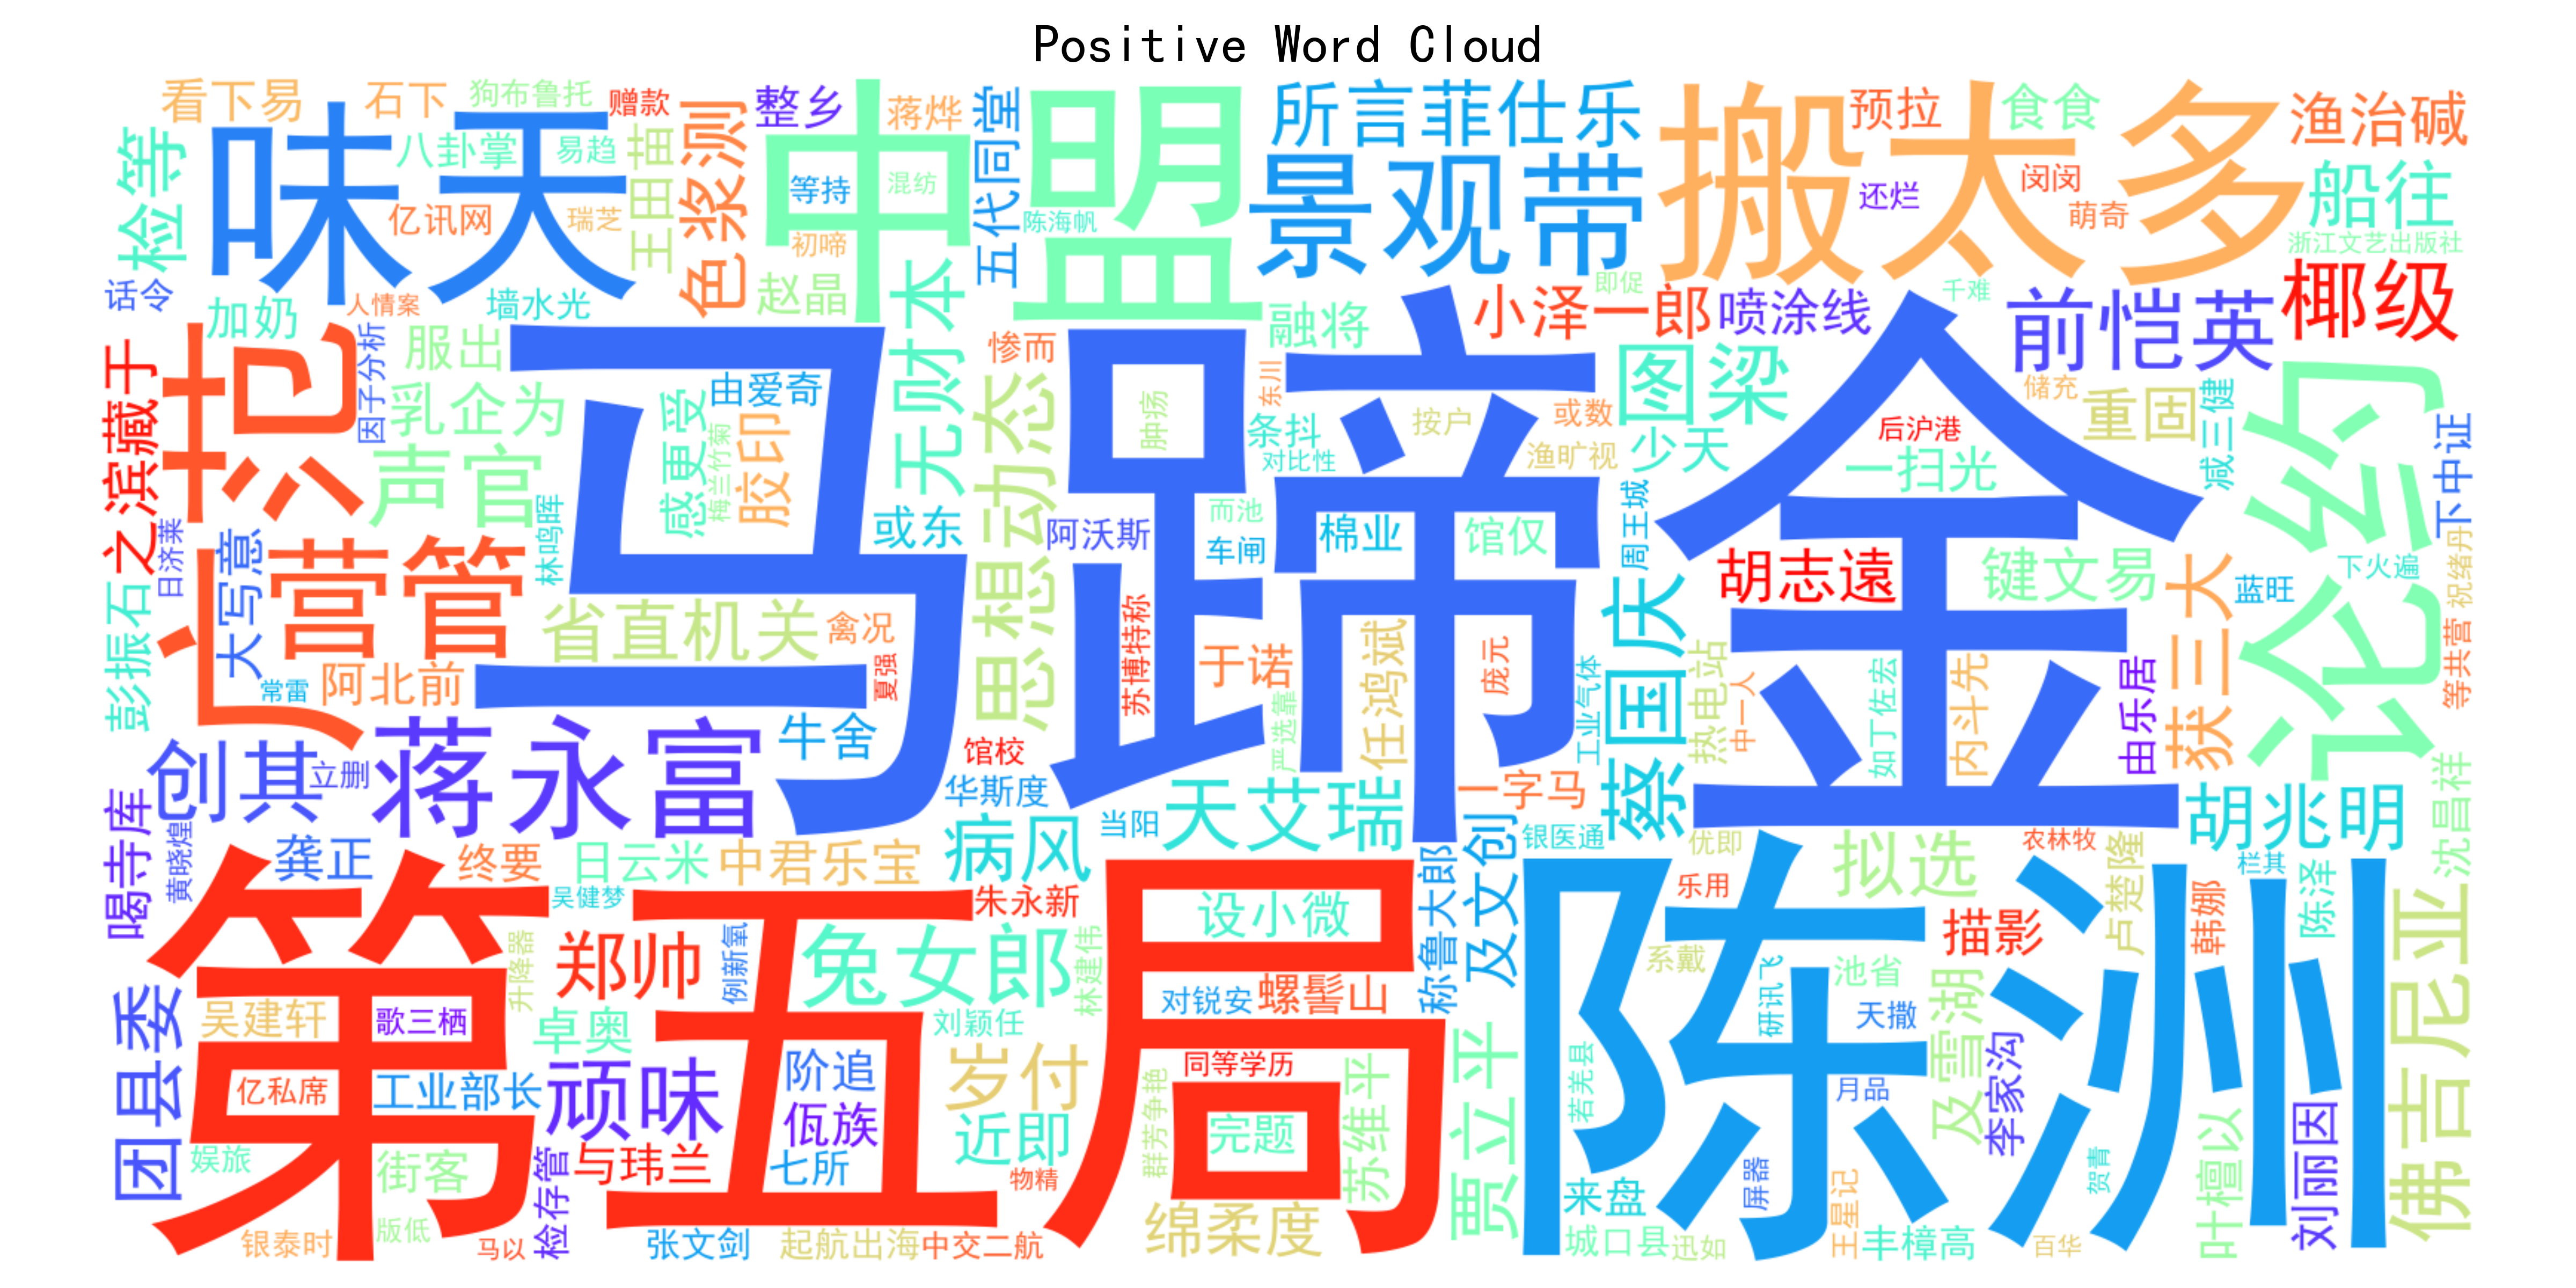
\includegraphics[width=0.63\linewidth]{wordcloud_positive.png}
      \caption{\small Positive Sentiment}

      \column{0.5\textwidth}
      \centering
      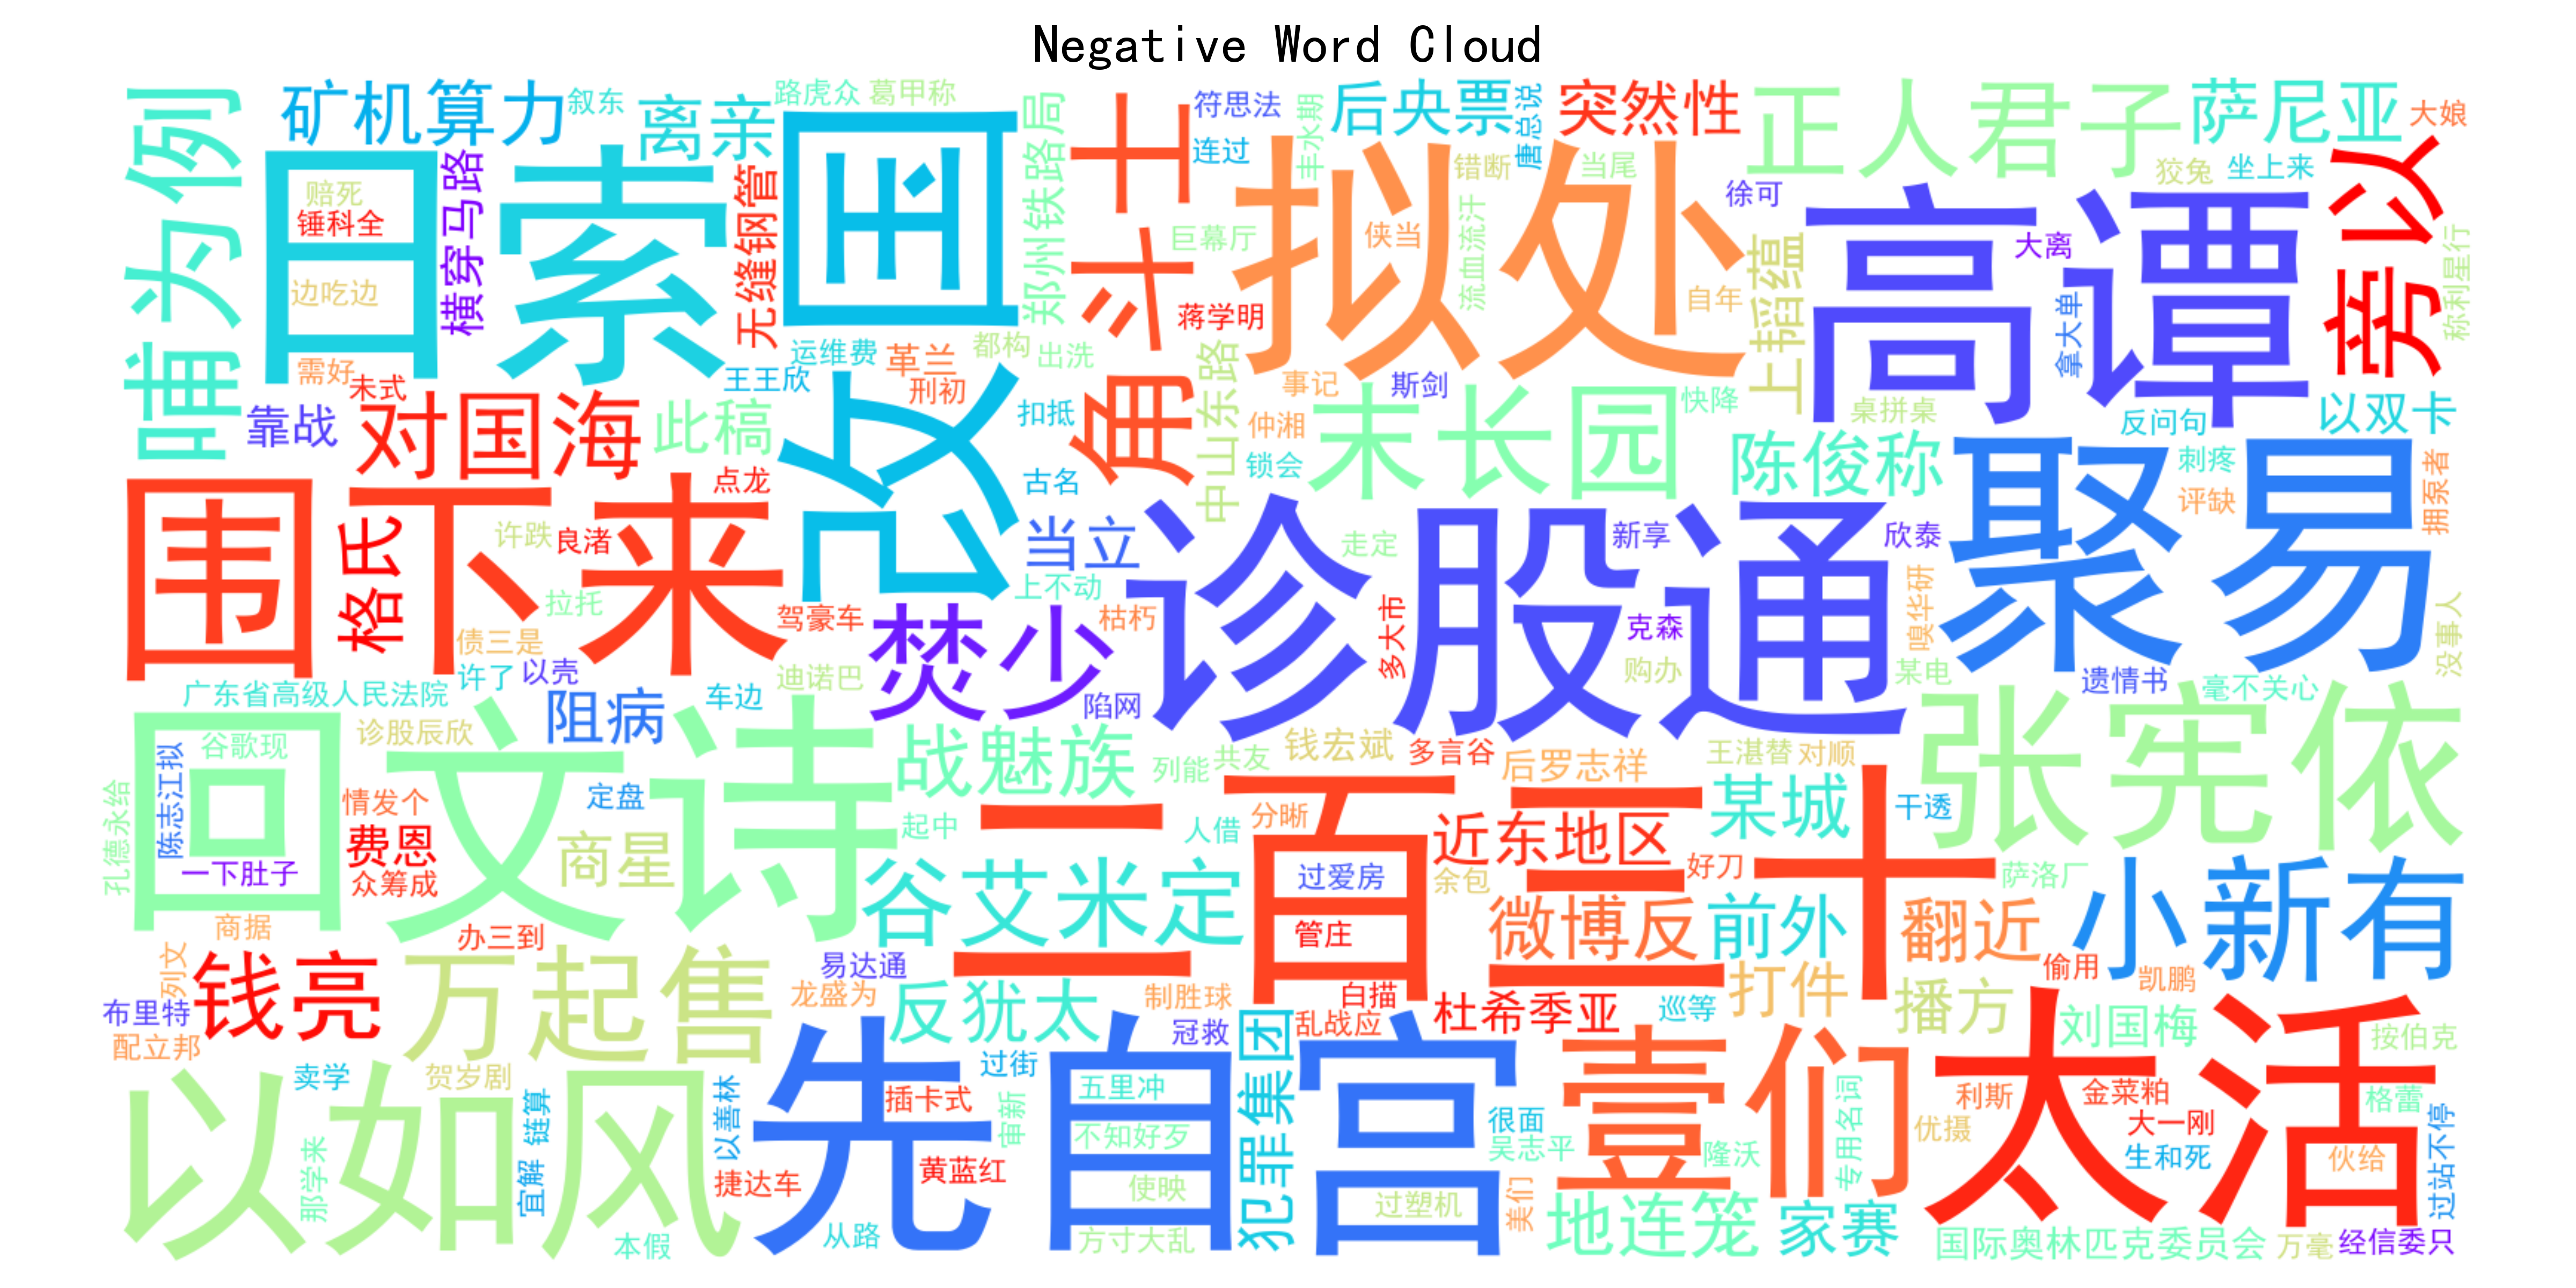
\includegraphics[width=0.63\linewidth]{wordcloud_negative.png}
      \caption{\small Negative Sentiment}
    \end{columns}
  \end{figure}
\end{frame}
  
\begin{frame}{Methods Overview}
  \textbf{1. Data Preparation and Augmentation:}
  \begin{itemize}
    \item Translate \underline{high-quality English financial sentiment corpora} into Chinese using a \underline{Transformer-based NMT model (TNMT)}.
    \item Result: \underline{Enlarged Chinese corpus} for sentiment analysis.
  \end{itemize}
  
  \textbf{2. Lexicon-Based Annotation:}
  \begin{itemize}
    \item Use a \underline{Chinese financial sentiment lexicon} for labeling, inspired by Jiang et al. (2019)\footnote{Jiang et al., \textit{J. Fin. Econ.}, 132(1), 126-149.}.
    \item Assign sentiments (positive, neutral, negative) via \underline{domain-specific terms}.
    \item Outputs: \underline{Automatically annotated Chinese dataset}.
  \end{itemize}
  
  \textbf{3. Model Training: BERT Fine-Tuning:}
  \begin{itemize}
    \item Fine-tune a \underline{pre-trained Chinese BERT model} with the annotated dataset.
    \item \underline{BERT captures contextual nuances}, surpassing traditional methods.
  \end{itemize}
  \end{frame}  

%-----------------------------------------------
% Results (5 slides)
%-----------------------------------------------
\begin{frame}{Results: Transformer-based NMT model (TNMT)}
  \textbf{Transformer Model Results:}
  \begin{figure}
    \centering
    % Top: Training Loss
    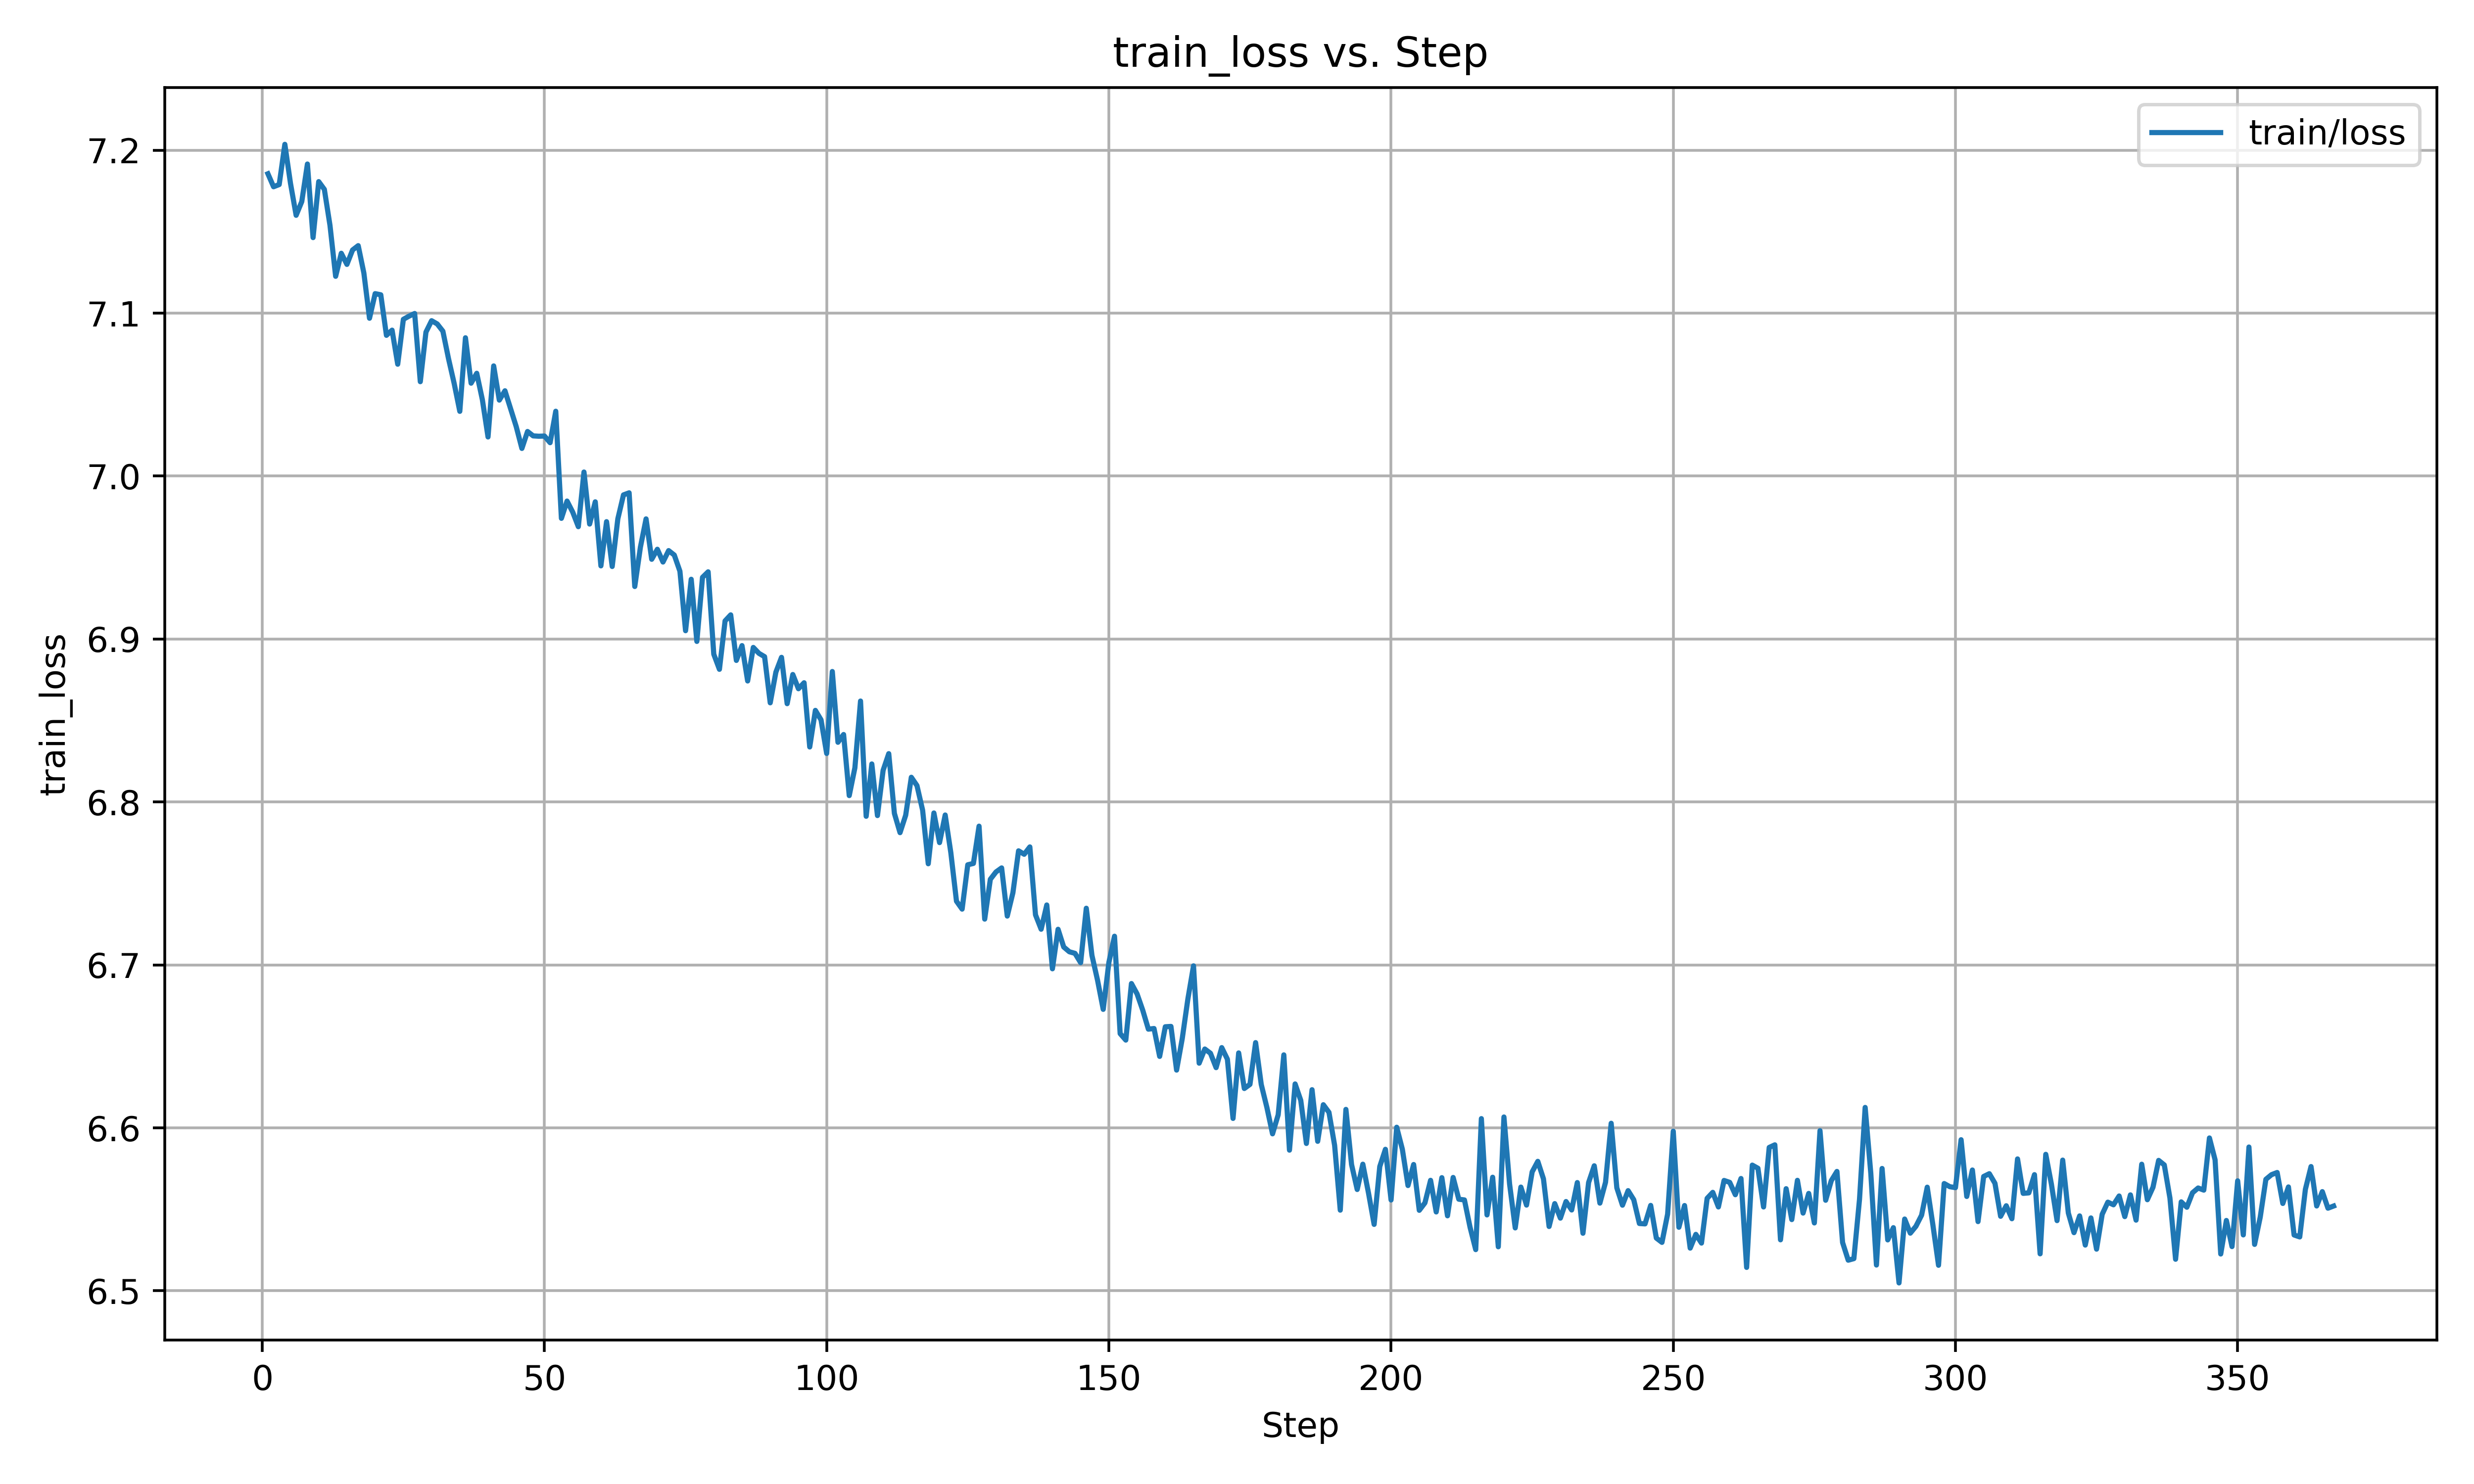
\includegraphics[width=0.25\linewidth]{Transformer_train_loss.png}
    \caption{\small Training Loss: 200 steps stable}
    \vspace{1em}

    % Bottom: BLEU Score and F1 Score side-by-side
    \begin{columns}[c]
      \column{0.5\textwidth}
      \centering
      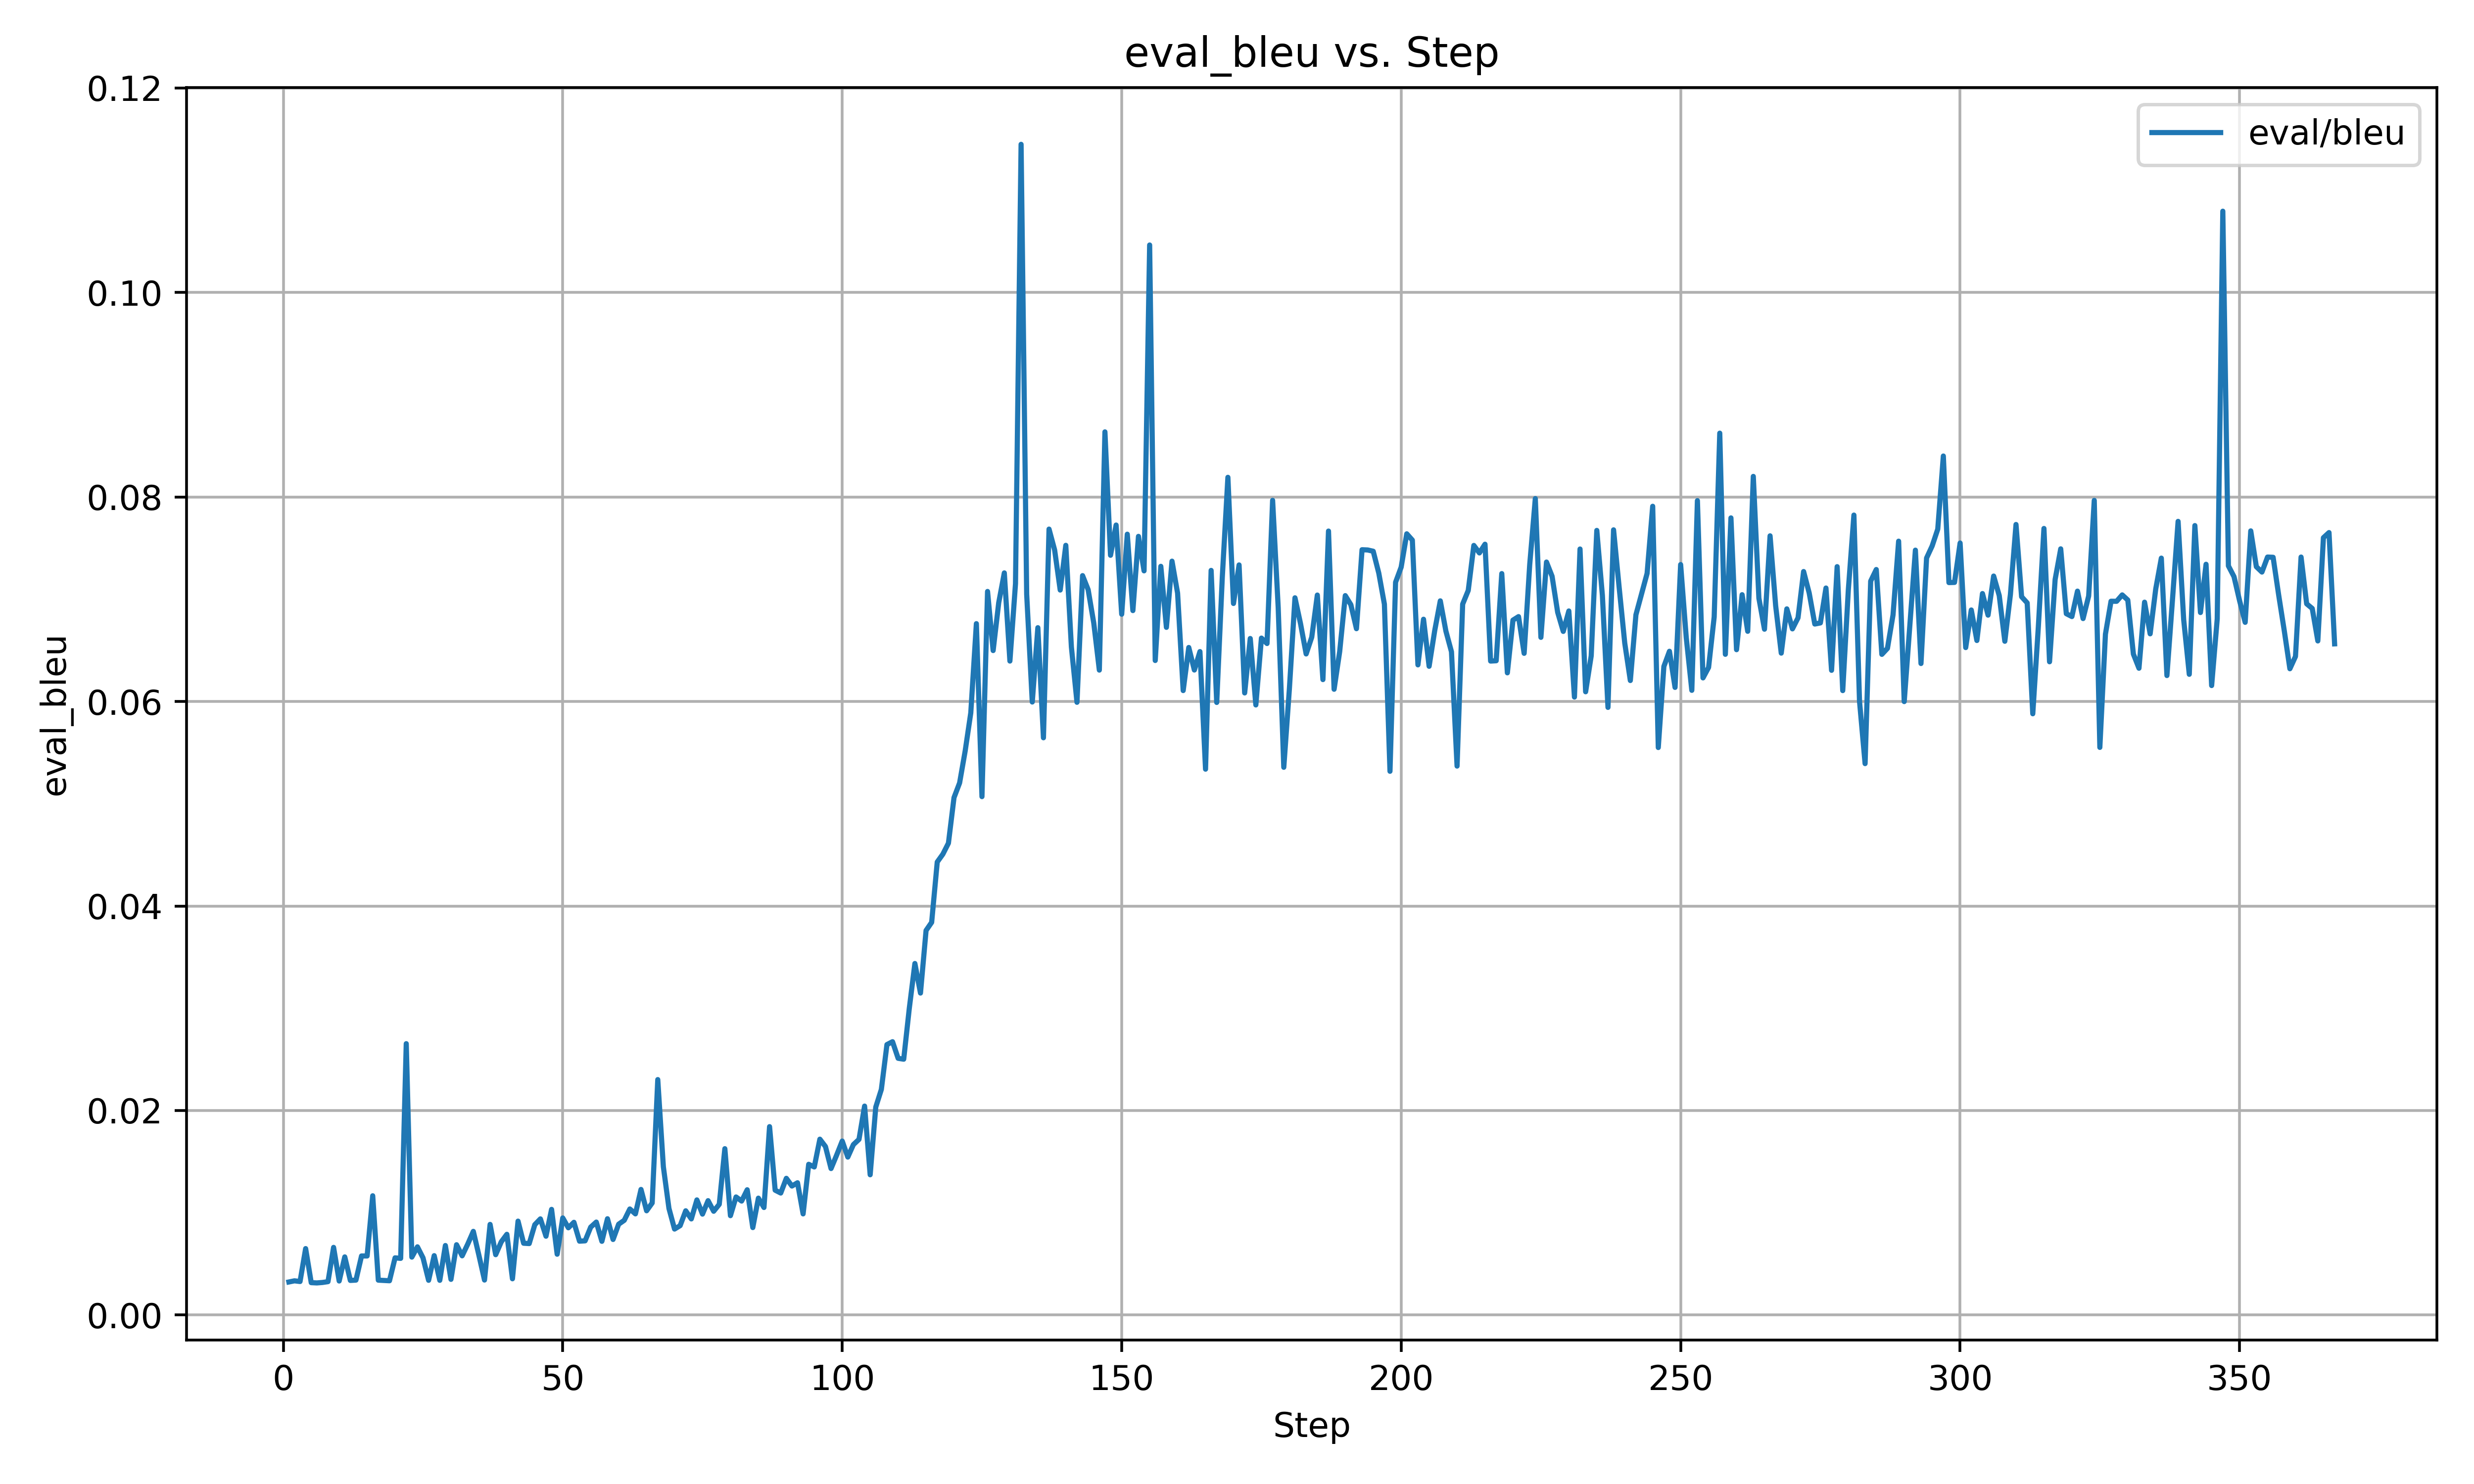
\includegraphics[width=0.55\linewidth]{Transformer_eval_bleu.png}
      \caption{\small Evaluation BLEU Score: 130 steps stable}

      \column{0.5\textwidth}
      \centering
      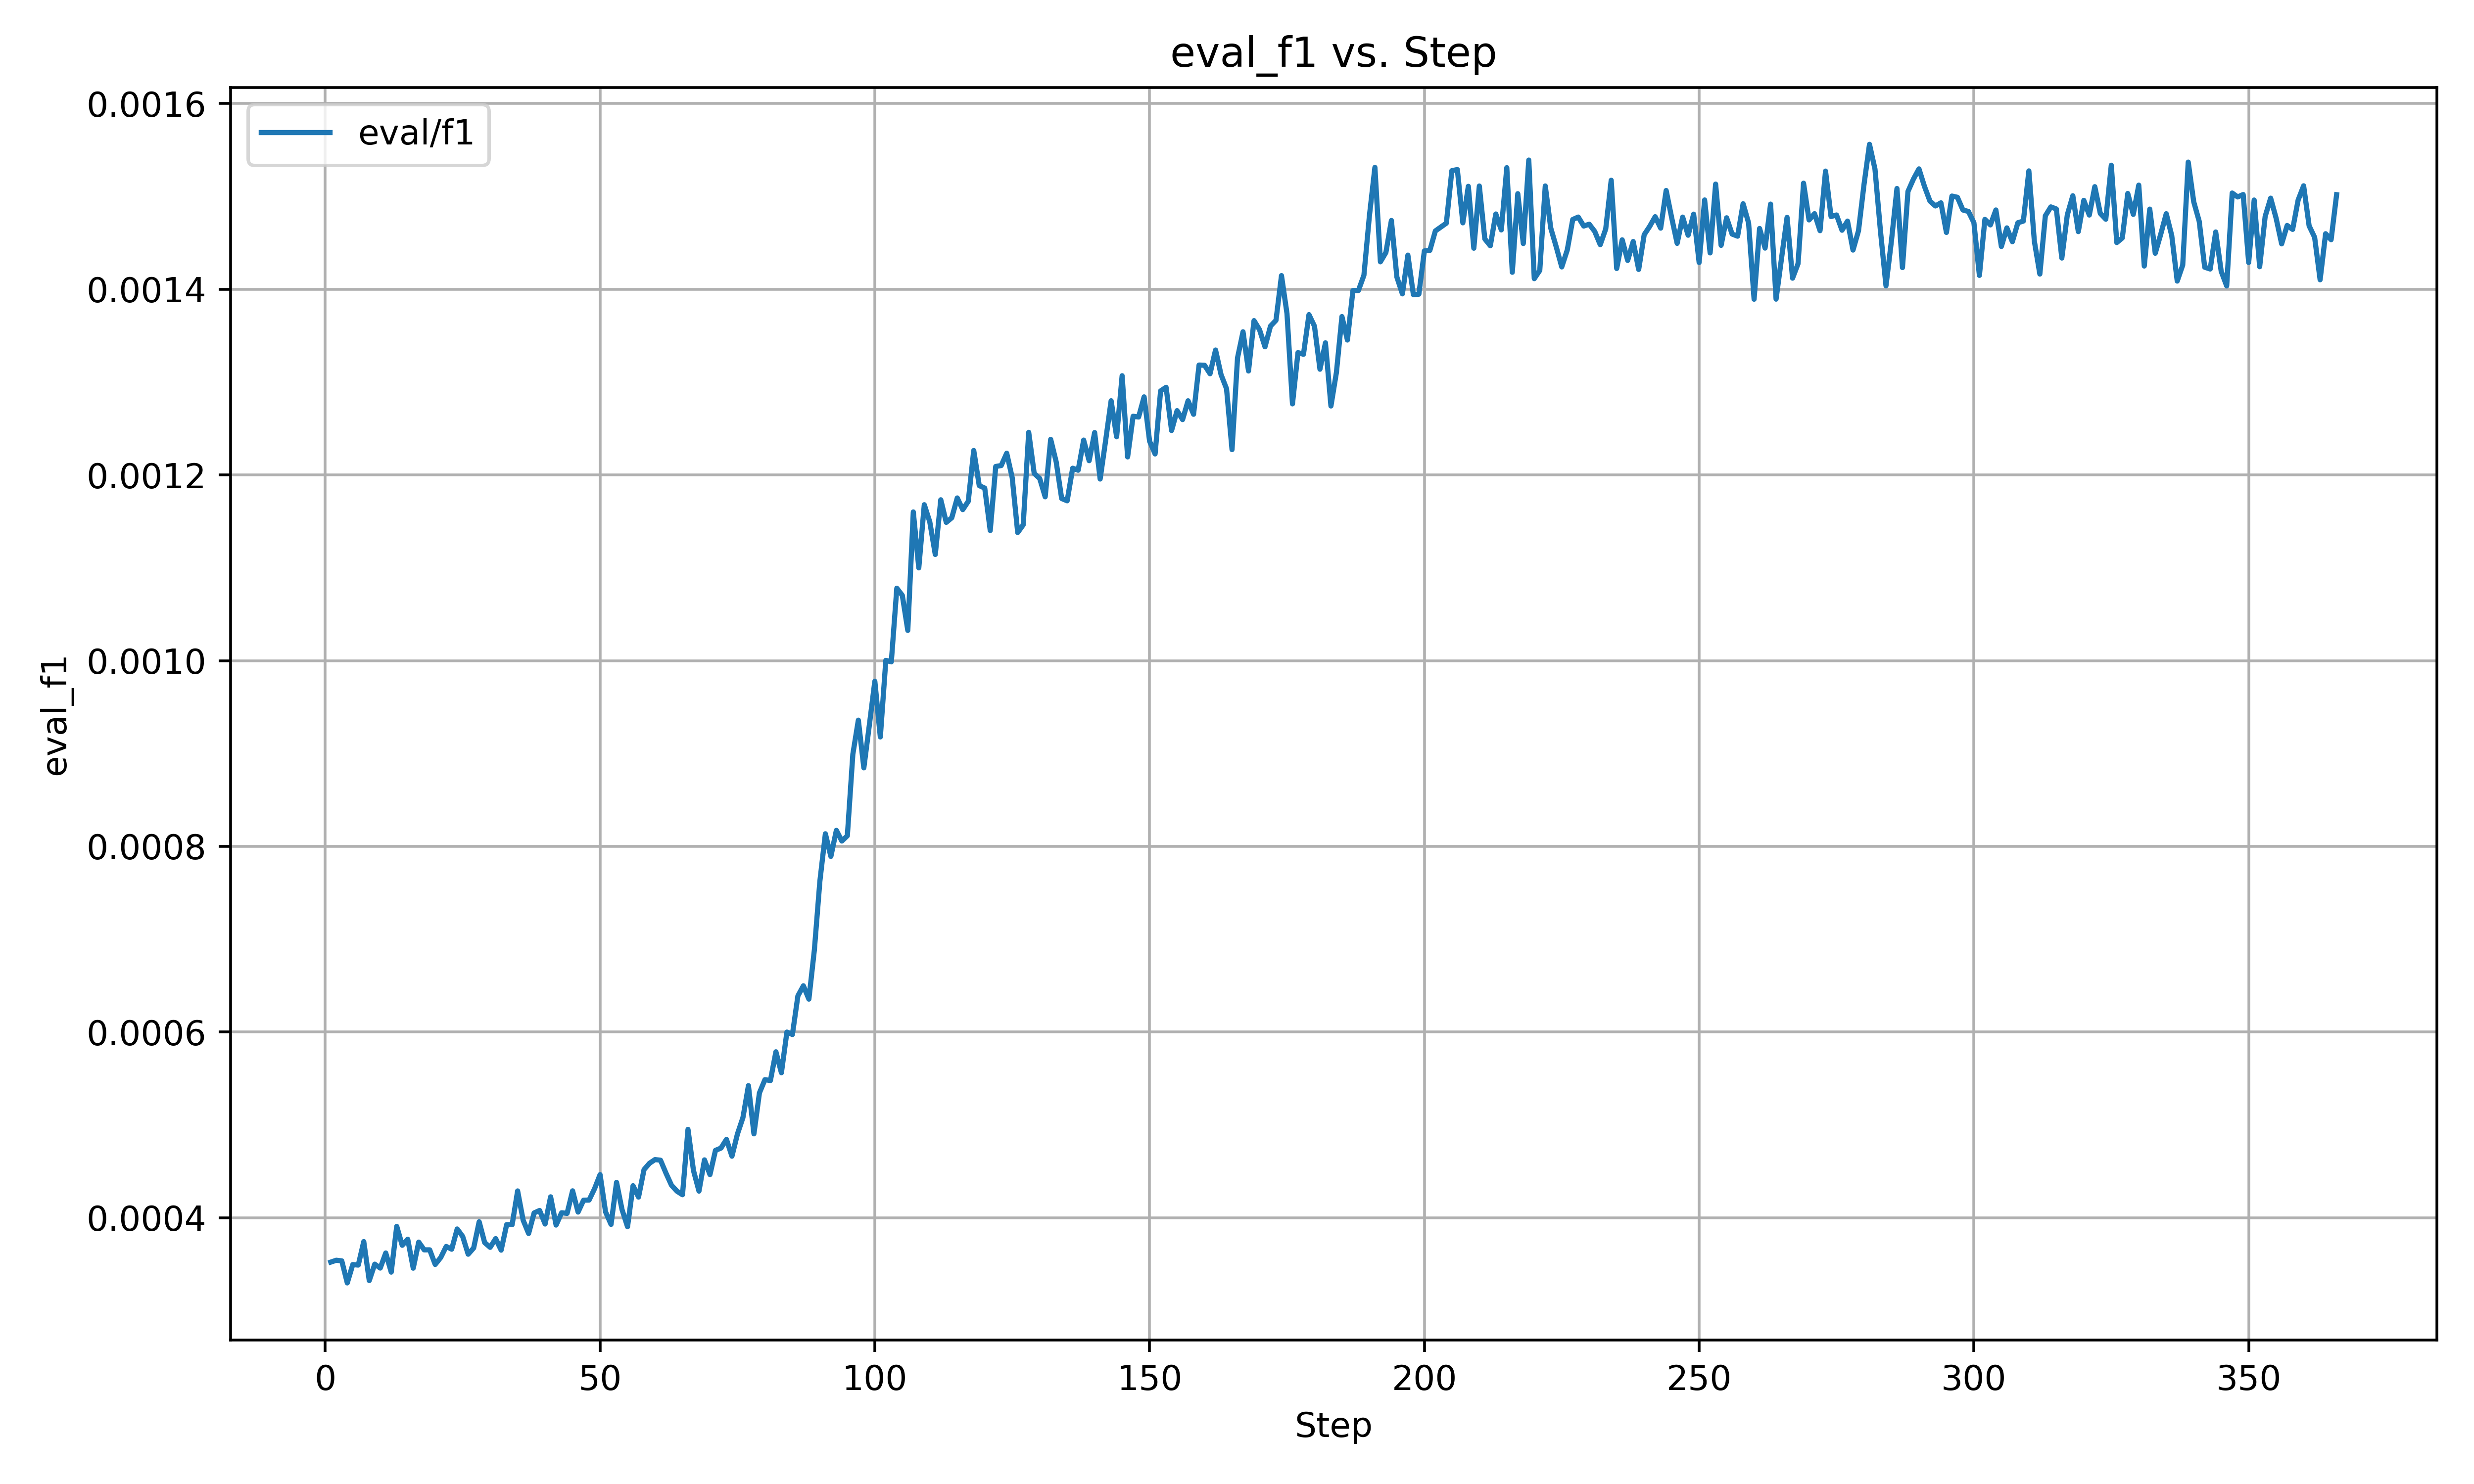
\includegraphics[width=0.55\linewidth]{Transformer_eval_f1.png}
      \caption{\small Evaluation F1 Score: 200 steps stable}
    \end{columns}
  \end{figure}
\end{frame}

\begin{frame}{Results: BERT Training}
  \textbf{BERT Model Training Results:}
  \begin{figure}
    \centering
    % Top: Training Accuracy
    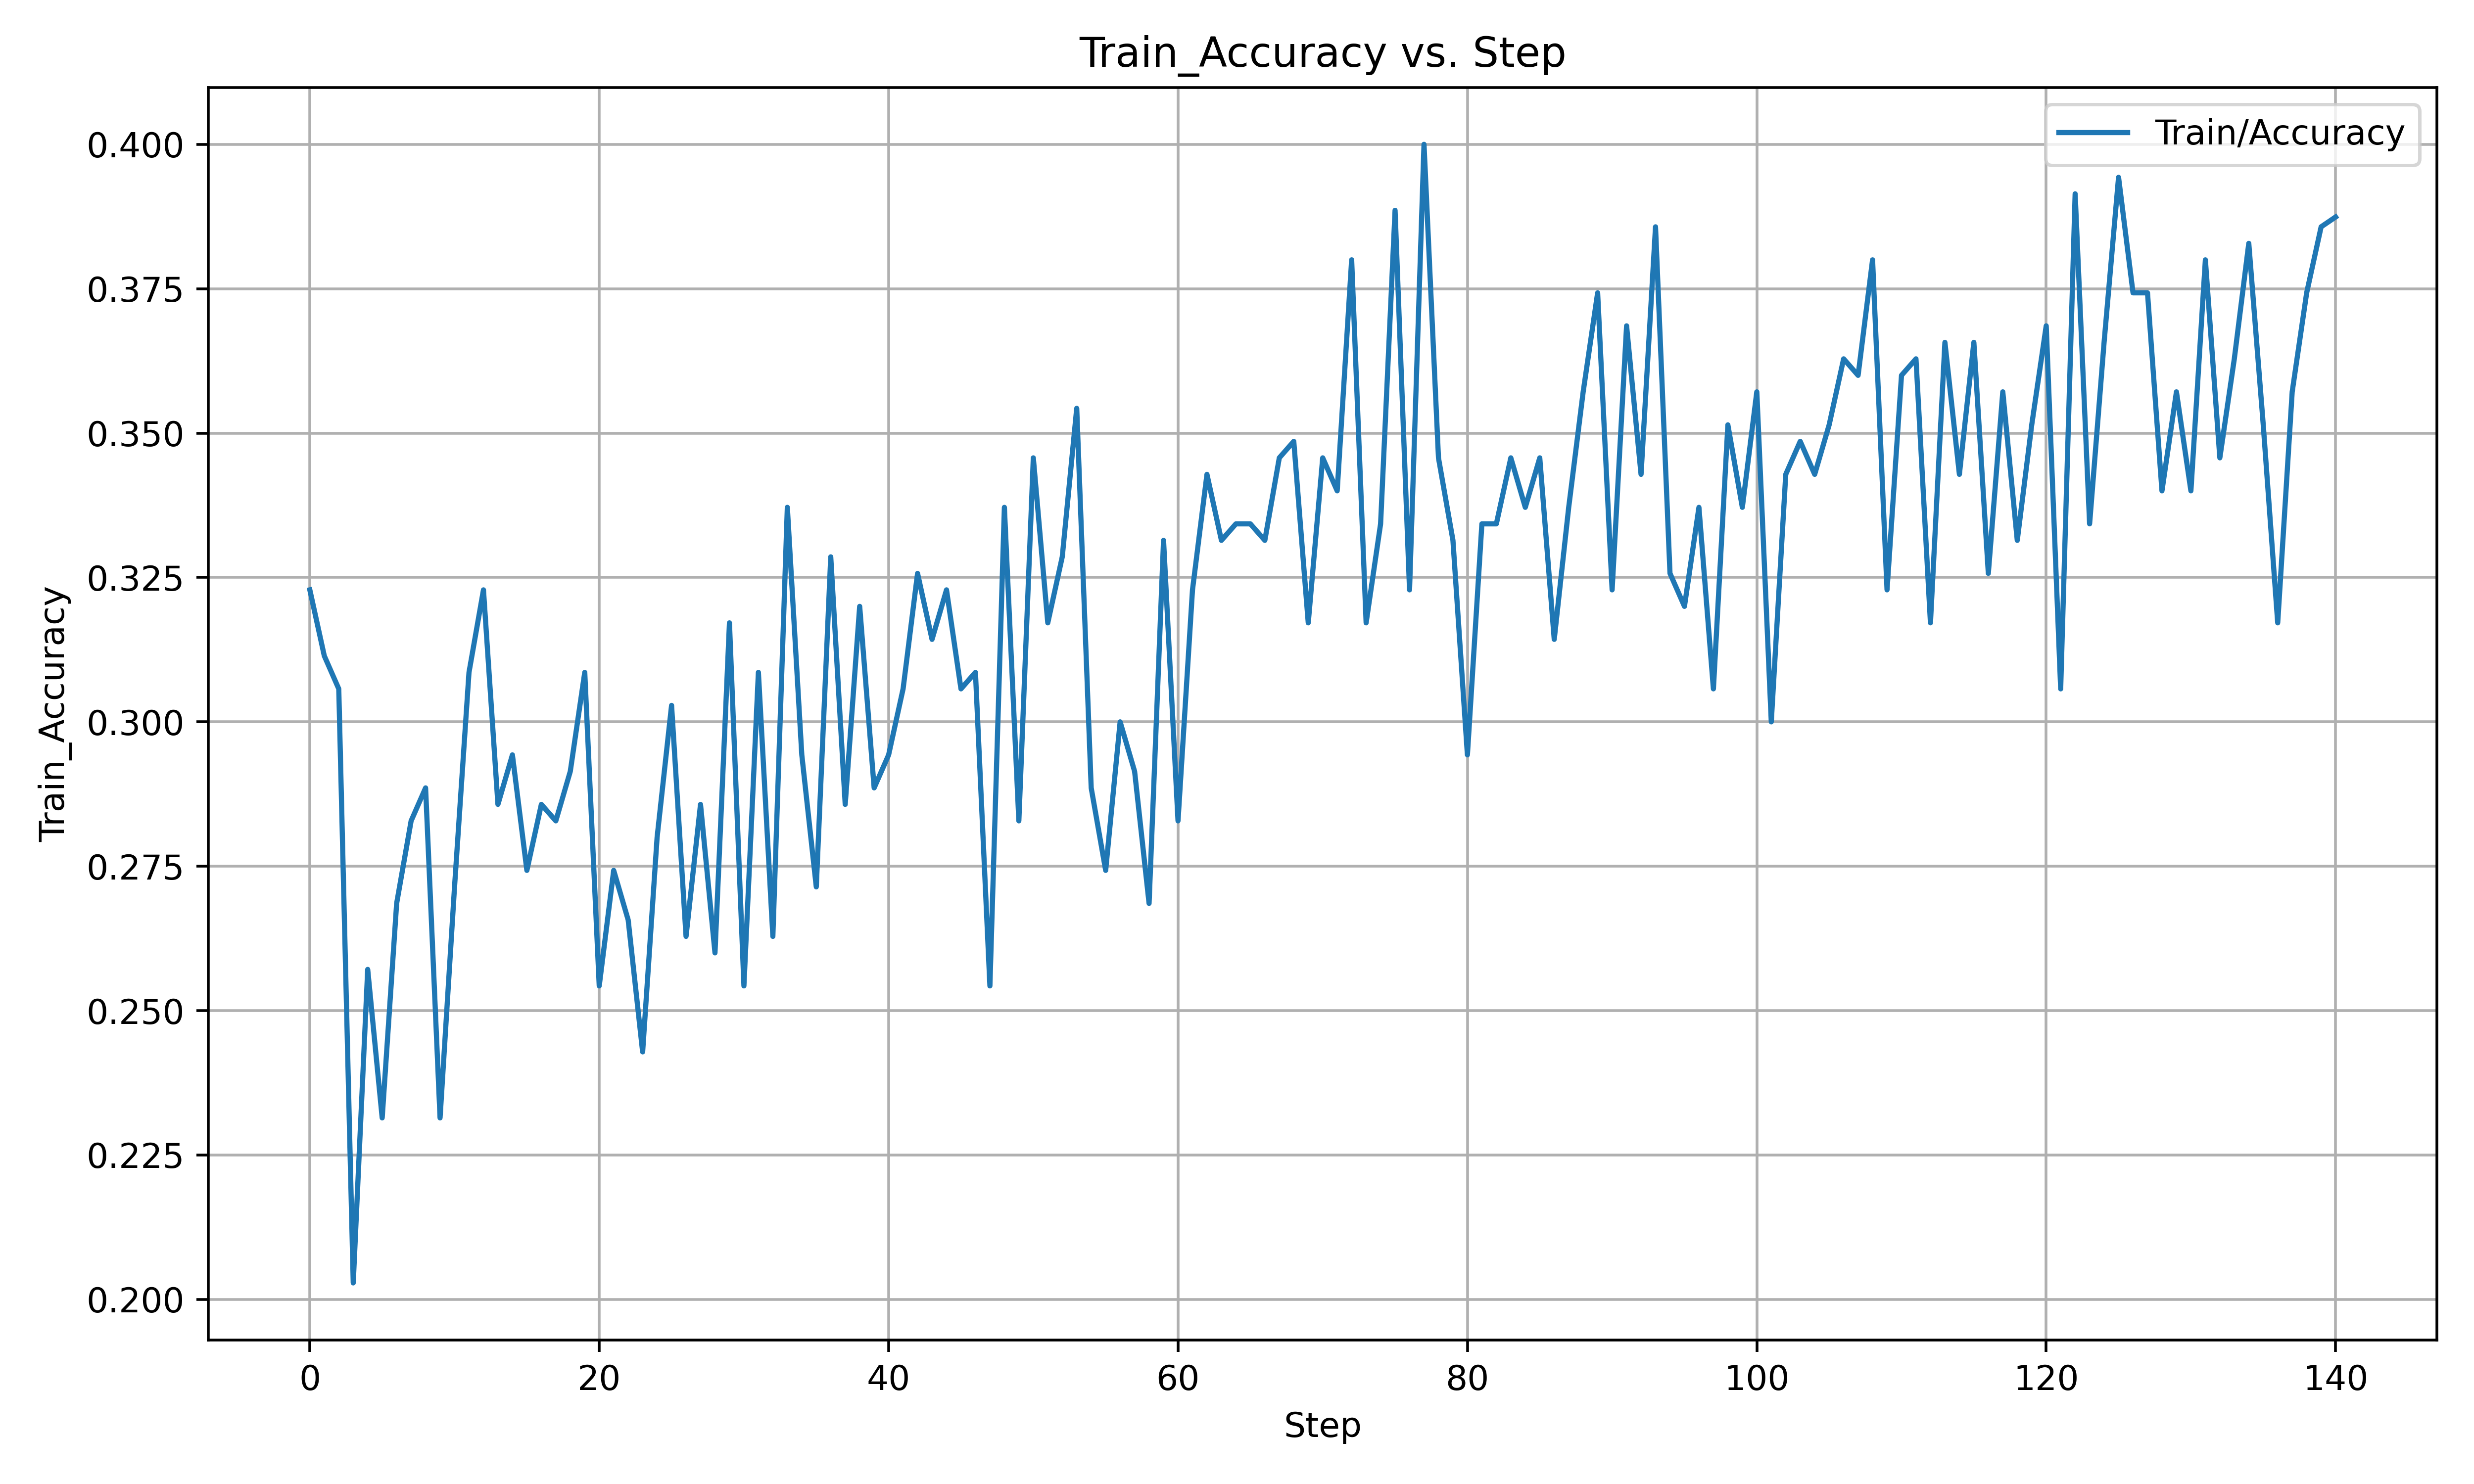
\includegraphics[width=0.25\linewidth]{BERT_Train_Accuracy.png}
    \caption{\small Training Accuracy: Increasing}
    \vspace{1em}

    % Bottom: F1 Score and Training Loss side-by-side
    \begin{columns}[c]
      \column{0.5\textwidth}
      \centering
      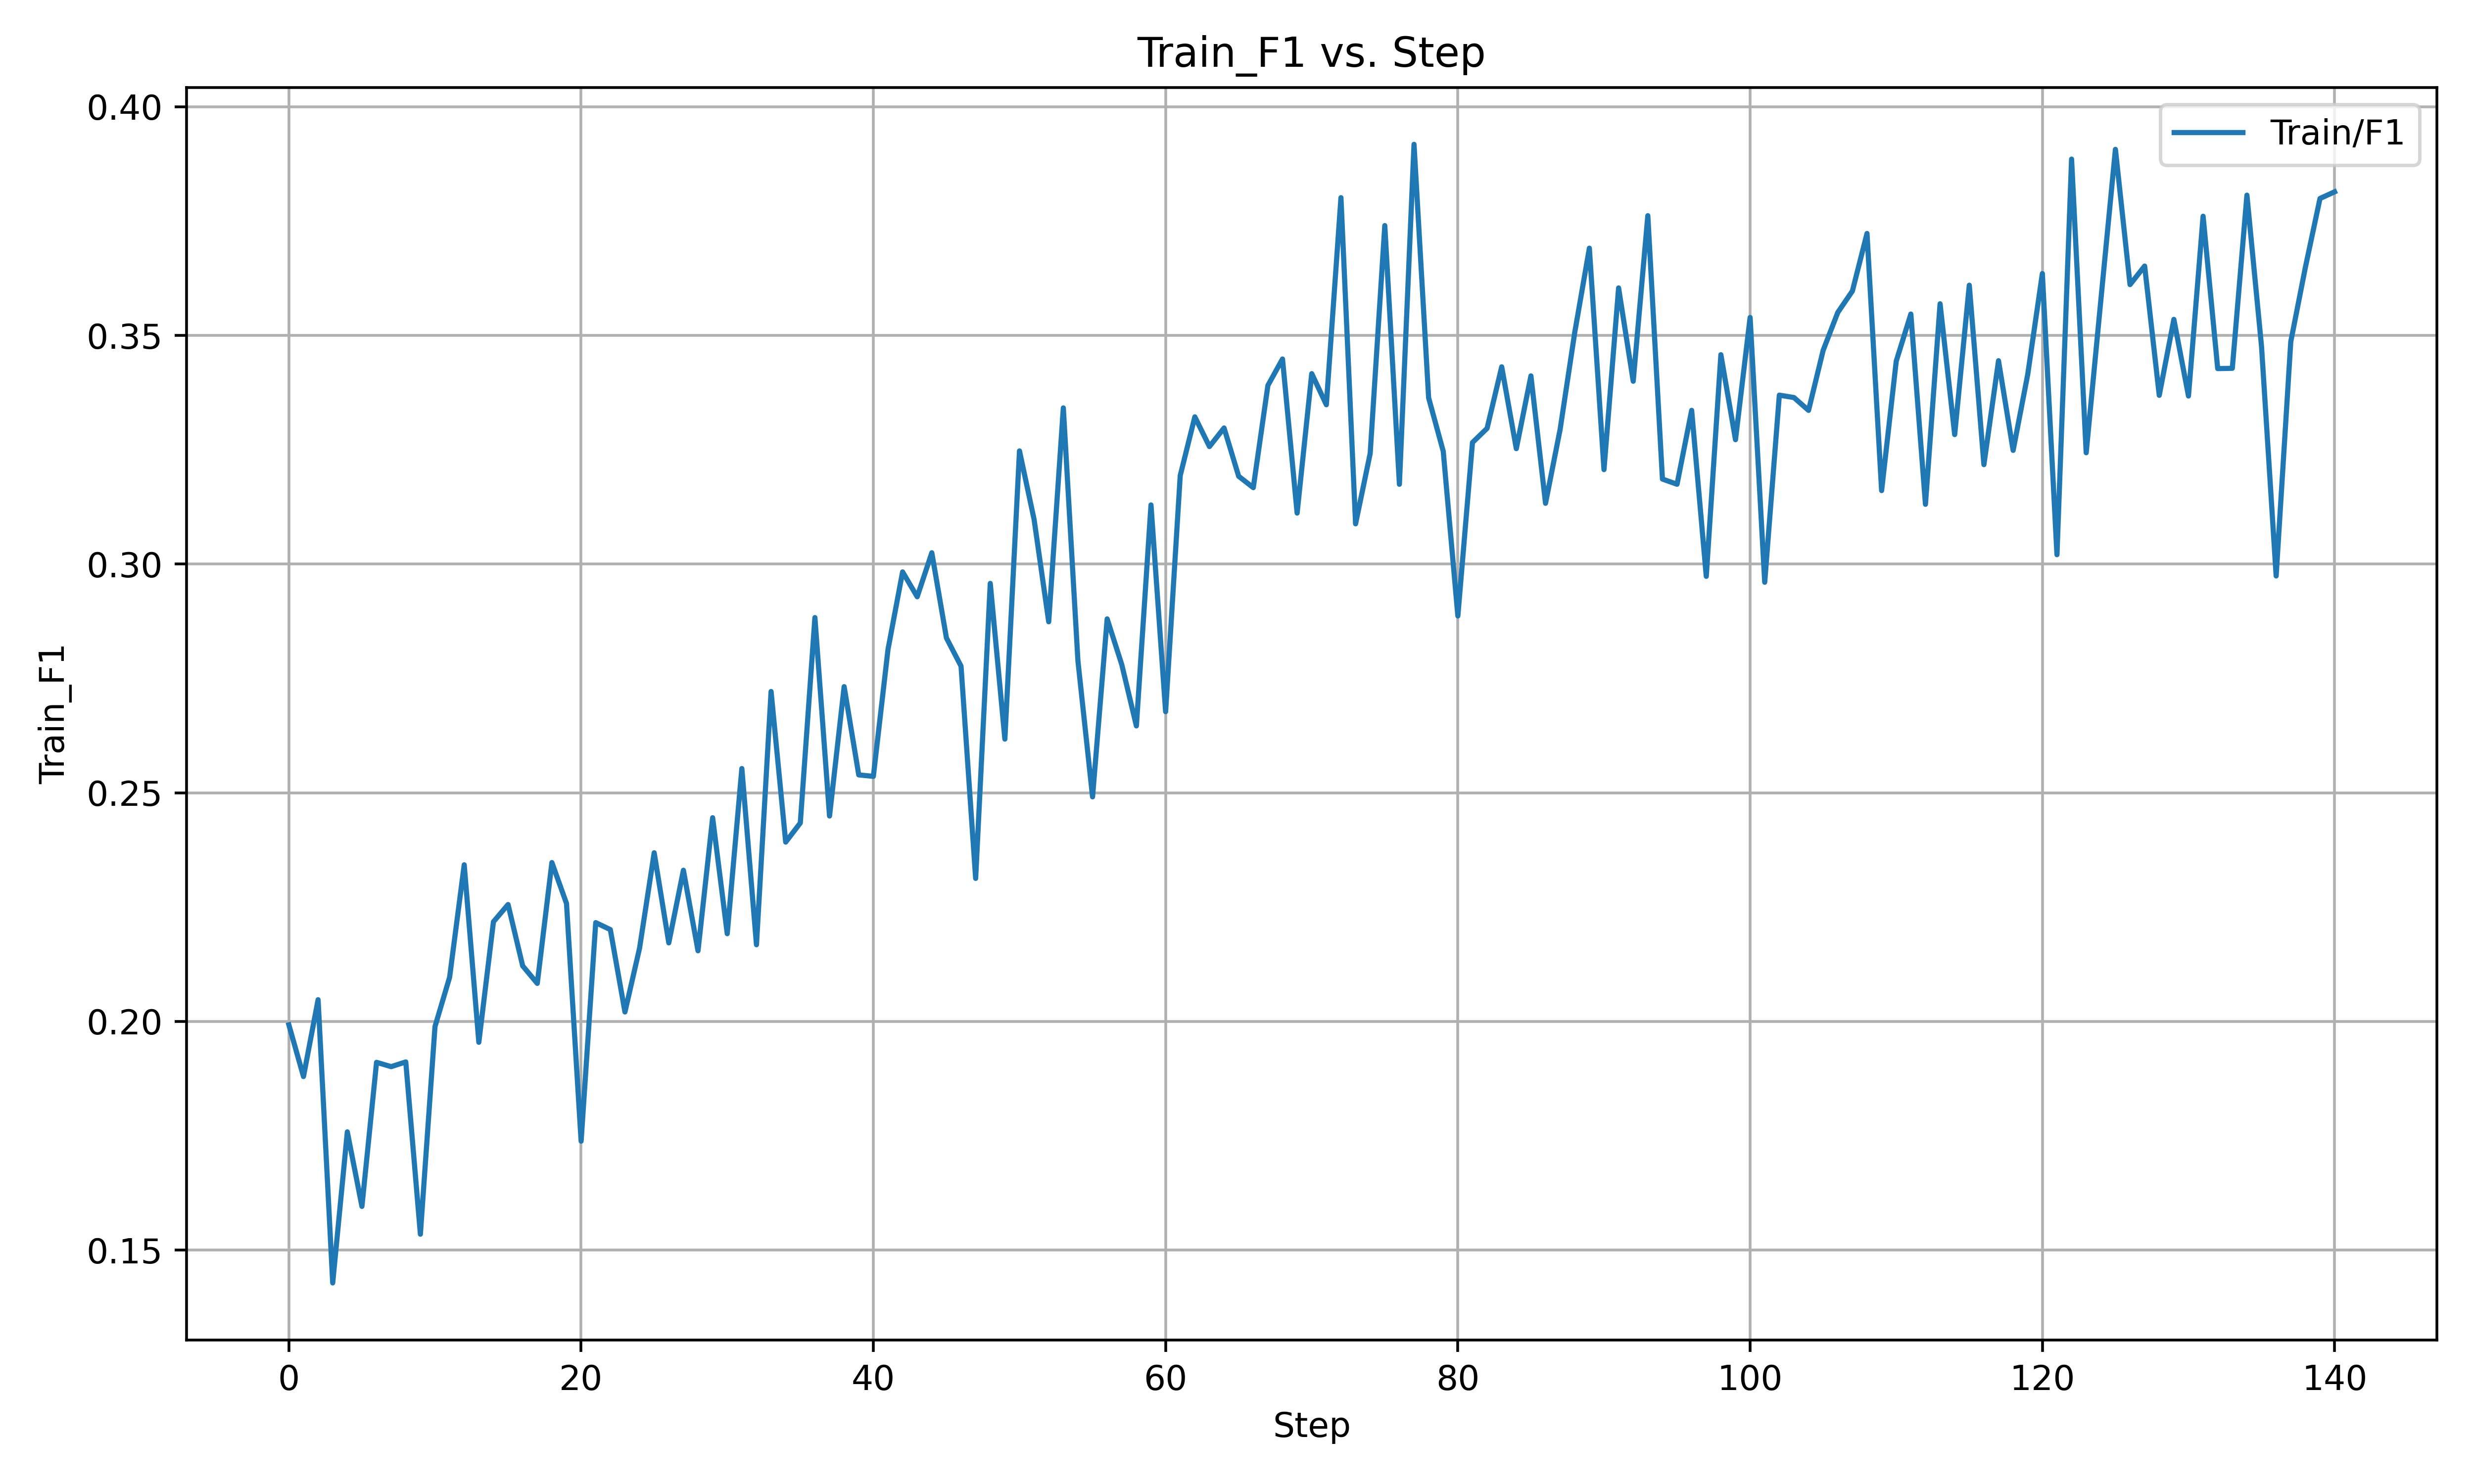
\includegraphics[width=0.55\linewidth]{BERT_Train_F1.png}
      \caption{\small Training F1 Score: 60 steps stable}

      \column{0.5\textwidth}
      \centering
      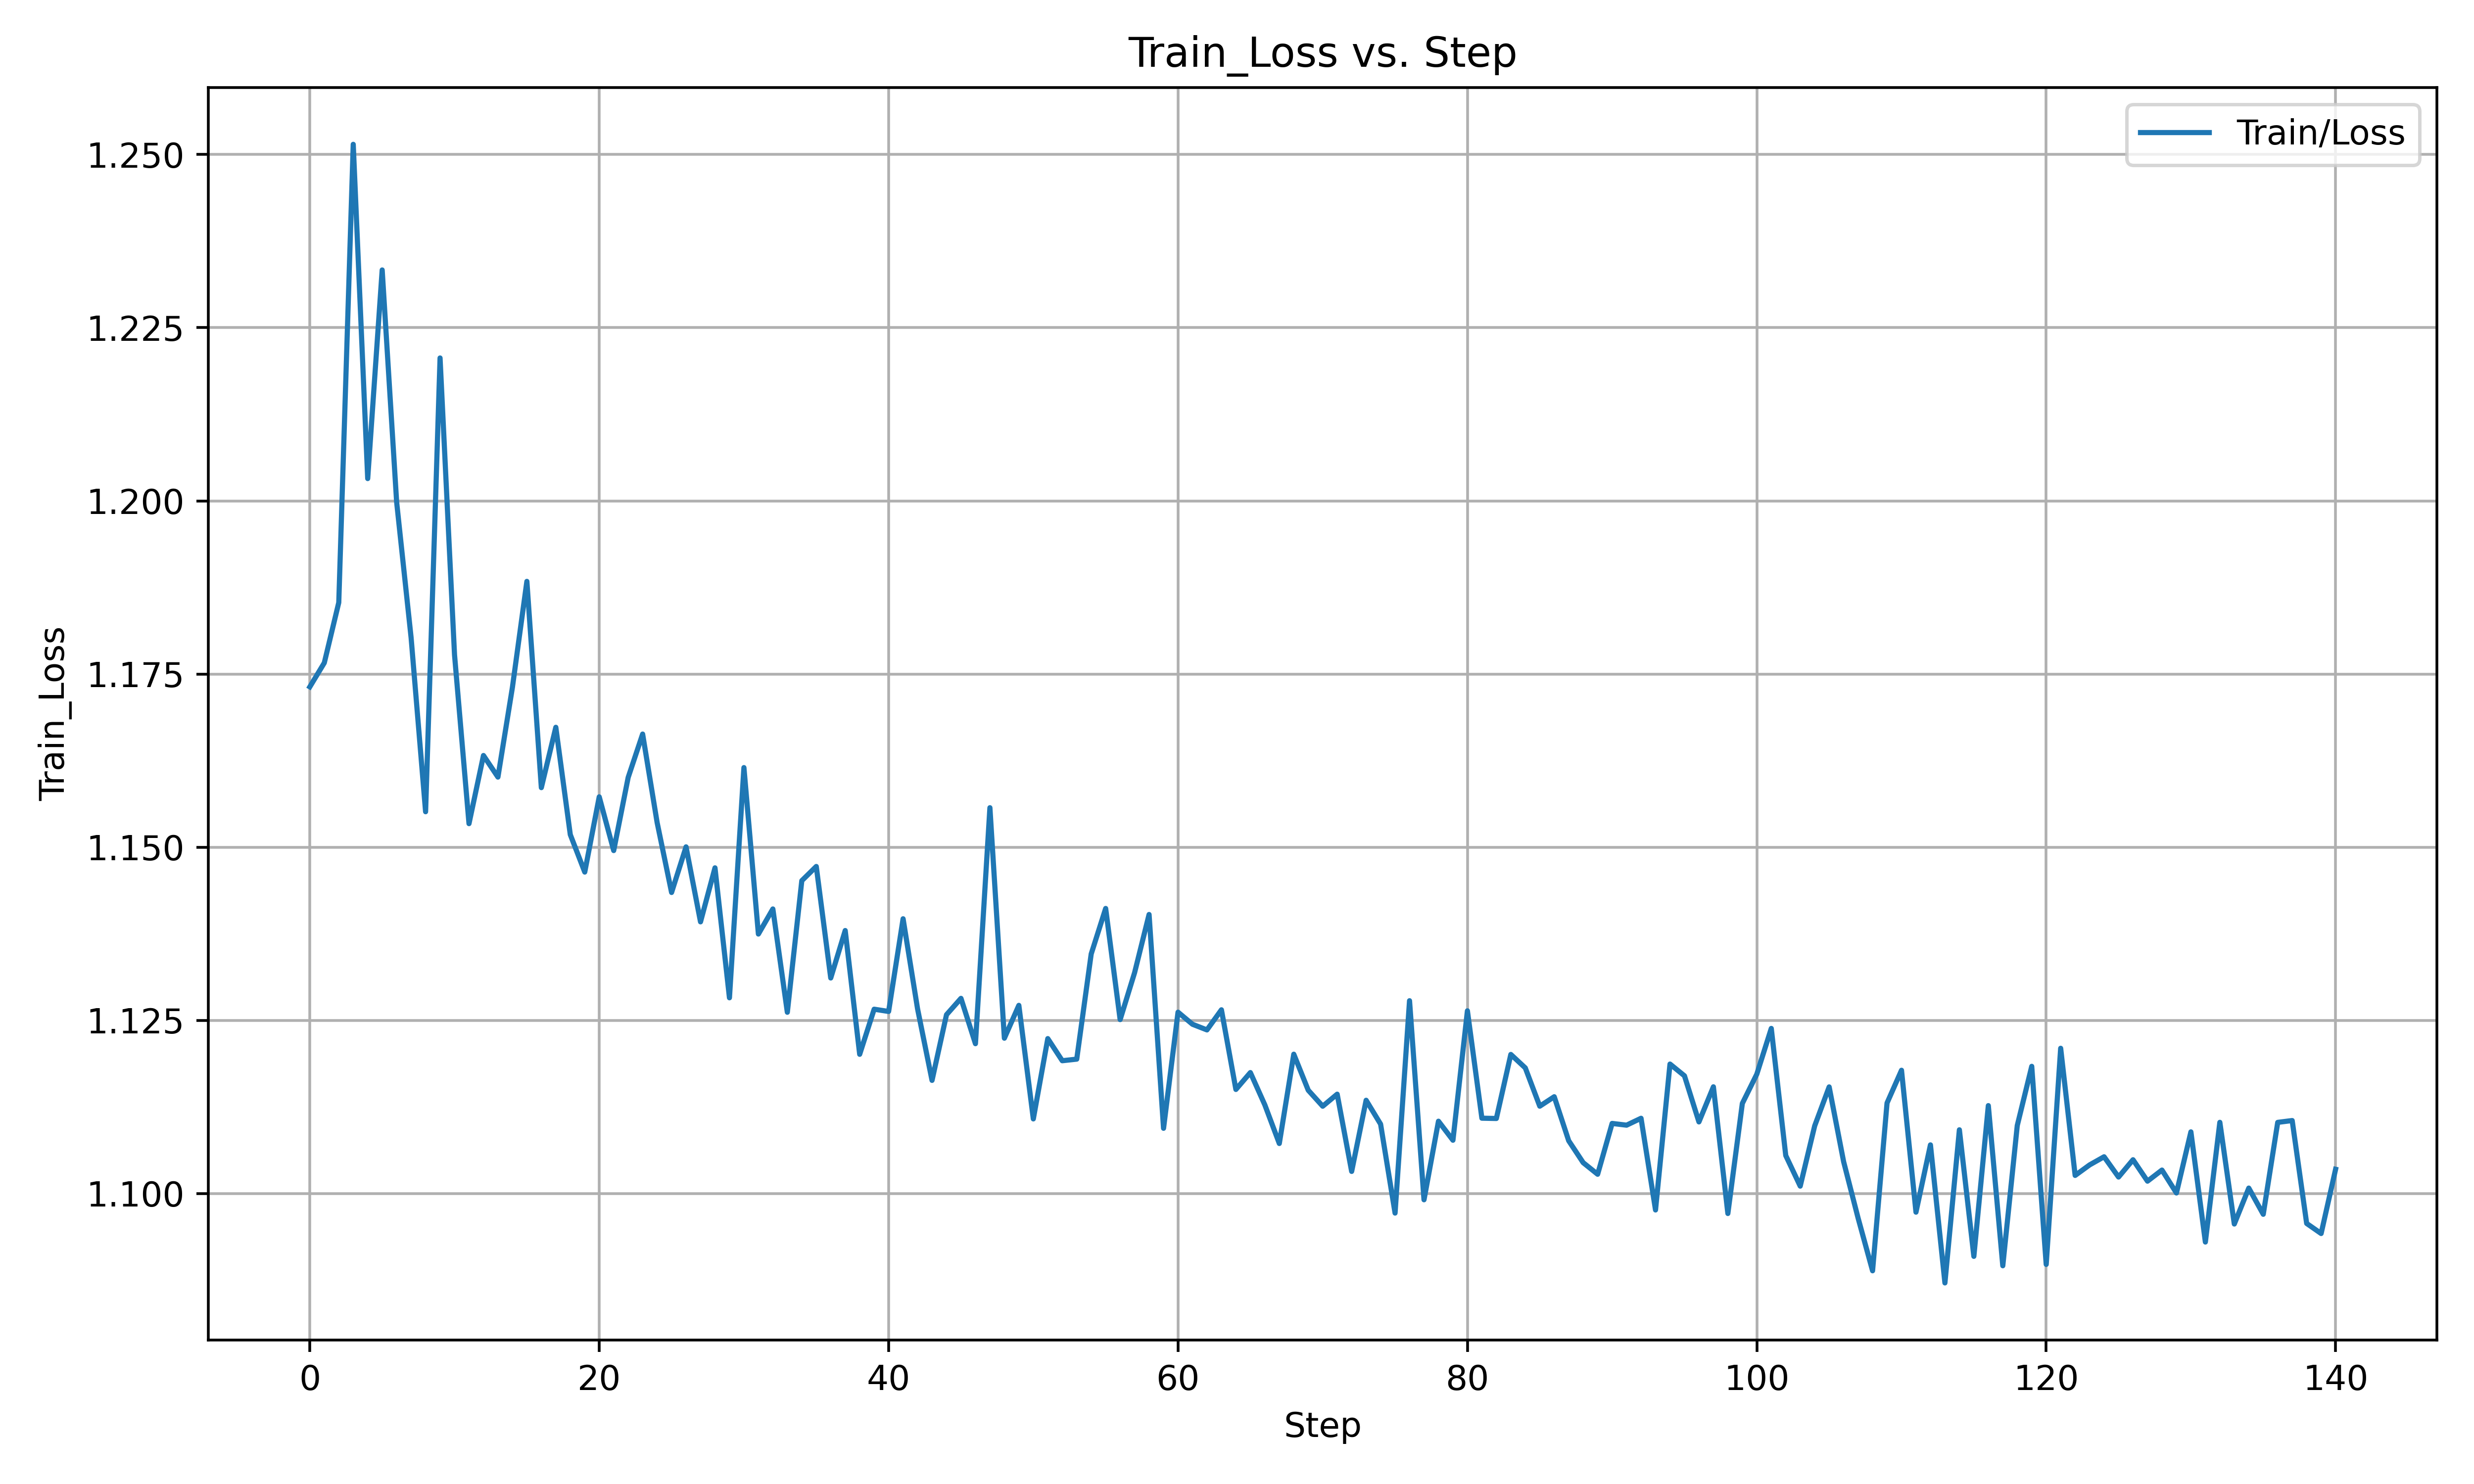
\includegraphics[width=0.55\linewidth]{BERT_Train_Loss.png}
      \caption{\small Training Loss: 120 steps stable}
    \end{columns}
  \end{figure}
\end{frame}

\begin{frame}{Results - Domain Adaptation}
  \begin{itemize}
    \item Effectively \underline{adapted English-origin sentiment cues to Chinese texts}.
    \item Enhanced \underline{model robustness in dynamic financial contexts}.
    \item Demonstrated \underline{scalable approach to other languages/domains}.
  \end{itemize}
\end{frame}

%-----------------------------------------------
% Conclusion (2 slides)
%-----------------------------------------------
\begin{frame}{Conclusions (1/2)}
\begin{itemize}
  \item Leveraged \underline{NMT to generate Chinese financial sentiment data from English corpora}.
  \item Applied \underline{lexicon-based annotation} to expand labeled datasets.
  \item Fine-tuned \underline{BERT to achieve improved classification performance}.
\end{itemize}
\end{frame}

\begin{frame}{Conclusions (2/2) - Resources}
\begin{itemize}
  \item \textbf{Video Presentation}: \underline{\url{https://example.com/video-demo}}
  \item \textbf{Code Repository}: \underline{\url{https://github.com/username/fin-sentiment-analysis}}
\end{itemize}
\end{frame}

\end{document}
